\documentclass[12pt]{article}
\usepackage[spanish, english, es-tabla]{babel}
\usepackage[utf8]{inputenc}
\usepackage[left = 2cm, right = 2cm, bottom = 2cm, top = 3cm]{geometry}
\usepackage{amsmath, amssymb}
\usepackage{graphicx}
\usepackage{hyperref}
\usepackage{listings}
\usepackage{courier}

\usepackage[dvipsnames]{xcolor}

\renewcommand{\lstlistingname}{Ejemplo}
\renewcommand{\lstlistlistingname}{Listado de ejemplos}

% https://tex.stackexchange.com/questions/60209/how-to-add-an-extra-level-of-sections-with-headings-below-subsubsection
\newcommand{\subsubsubsection}[1]{\paragraph{#1}\mbox{}\\}
\setcounter{secnumdepth}{4}
\setcounter{tocdepth}{4}

% Configure lstlisting
\definecolor{codegreen}{rgb}{0,0.6,0}
\definecolor{codegray}{rgb}{0.5,0.5,0.5}
\definecolor{codepurple}{rgb}{0.58,0,0.82}
\definecolor{backcolour}{rgb}{0.95,0.95,0.92}

\lstdefinestyle{mystyle}{
	backgroundcolor=\color{backcolour},   
	commentstyle=\color{codegreen},
	keywordstyle=\color{magenta},
	numberstyle=\tiny\color{codegray},
	stringstyle=\color{codepurple},
	basicstyle=\ttfamily\footnotesize,
	breakatwhitespace=false,         
	breaklines=true,                 
	captionpos=t,                    
	keepspaces=true,                 
	numbers=left,                    
	numbersep=5pt,                  
	showspaces=false,                
	showstringspaces=false,
	showtabs=false,                  
	tabsize=2
}

\lstset{style=mystyle}

\begin{document}
	\selectlanguage{spanish}
	
	%%%% PORTADA
	\title{\textbf{Aplicación de técnicas de virtualización ligera para la evaluación de redes de comunicaciones} \\ 
	\addvspace{10px} \large \textit{Trabajo Final de Estudios} \\
	\large Ingeniería Telemática}
	\author{Autor: Enrique Fernández Sánchez \\ Tutor: Josemaria Malgosa Sanahuja \\ \\Universidad Politécnica de Cartagena}
	
	%% EDITAR PARA SEGUIMIENTO DE VERSIONES
	\date{Revisión Octubre 2021}
	
	\maketitle
	
	%%% END PORTADA
	
	\pagebreak
	
	\tableofcontents
	
	\pagebreak
	
	\addcontentsline{toc}{section}{Índice de figuras}
	\listoffigures
	\addcontentsline{toc}{section}{Índice de tablas}
	\listoftables
	\addcontentsline{toc}{section}{Listado de ejemplos}
	\lstlistoflistings
	
	\pagebreak
	
	%%% Glosario
	\pagebreak
	\section*{Glosario de términos}
	\addcontentsline{toc}{section}{Glosario de términos}
	
	\noindent{\large \textbf{NFV} (\textit{Network Function Virtualization})}. \textit{Network Function Virtualization}, o bien, Virtualización de funciones de red.\\
		 
	\noindent{\large \textbf{SDN} (\textit{Software Defined Networks})}\\
		 
	\noindent{\large \textbf{Namespace}}. \textit{Espacio de nombres}\\
		 
	\noindent{\large \textbf{NS} (\textit{Network namespace})}. Tipo de espacio de nombres en Linux que tiene por función aislar la parte de red de la máquina host.\\
	
	\noindent{\large \textbf{Linux}}. Sistema operativo tipo UNIX, de codigo abierto, multiplataforma, multiusuario y multitarea.\\
	
	\noindent{\large \textbf{Unix}}. Sistema operativo portable, multitarea y multiusuario desarrollado a partir de 1969. Se divide en tres tareas básicas: el nucleo de sistema operativo, el interprete de comandos y programadas de utilidades.  \\
		 
	\noindent{\large \textbf{Kernel de Linux}}. Núcleo del sistema operativo Linux.\\
		 
	\noindent{\large \textbf{PID} (\textit{Process Identifier})}. Identificador de procesos que están ejecutándose bajo un sistema tipo Linux.\\
	
	\noindent{\large \textbf{UID} (\textit{User identifier})}. Encontrado normalmente como un número o palabra, supone un identificador de usuario dentro del sistema Linux.\\
	
	\noindent{\large \textbf{GID} (\textit{Group Identifier})}. Al igual que sucede con el UID, suele aparecer como un número o palabra y hace referencia al identificador de grupo dentro del sistema de Linux.\\
		 
	\noindent{\large \textbf{root}}. Cuenta superusuario del sistema operativo Linux.\\
		 
	\noindent{\large \textbf{veth-pair} (\textit{Virtual Ethernet Pair})}. Tipo de interfaz virtual. Funcionan de dos en parejas.\\
		 
	
	\pagebreak
	
	%%% TODO
	\section*{Agradecimientos}
	\addcontentsline{toc}{section}{Agradecimientos}
	
	\pagebreak
	
	%%% TODO
	\section{Introducción}
	\noindent Con el fin de concluir los estudios de grado en ingeniería telemática, es necesaria la investigación y el posterior desarrollo del \textit{Trabajo Fin de Estudios} (TFE). Dicho trabajo, tiene como objetivo enfrentar al alumno a un proceso de investigación en el que pueda aplicar los conceptos que ha ido aprendiendo durante su paso por el grado, además pudiendo añadir puntos de innovación, y aportar soluciones nuevas a un proyecto en específico.\\
	
	\noindent En este documento, recojo lo que sería mi memoria en relación al TFE. En dicho documento detallaremos las diferentes investigaciones realizadas sobre el concepto de virtualización en sistemas Linux, como funcionan los contenedores y como utilizar la virtualización ligera para la evaluación de redes de comunicaciones, en nuestro caso, de conmutación de paquetes.
	
	\subsection{Contexto del trabajo}
	\noindent Este proyecto nace con el objetivo de profundizar en conceptos novedosos para el ámbito de red, como por ejemplo podría ser NFV. Definimos NFV (Network Function Virtualization) como la virtualización de hardware físico de red, con el fin de solucionar problemas de escalabilidad y de optimización.\\
	
	 \noindent Además, trabajaremos sobre otras tecnologías igual de importantes como pueden ser la virtualización de recursos, o los bien conocidos \textit{contenedores}. Particularizaremos estas tecnologías y las acercamos al campo de conocimiento de la telemática para utilizarlas con el fin de evaluar y simular redes de conmutación de tipo IP. \\
	
	\noindent Partiendo de supuesto de que las herramientas más sencillas de simulación de redes se nos pueden quedar cortas en cuanto queremos escalar el sistema, nos topamos en que otras soluciones pueden ser mucho más \textit{resource hungry} de lo que podríamos imaginar. Además, tampoco podemos contar con realizar dichas pruebas de manera física, ya que el presupuesto del proyecto escalaría de nivel exponencial. Esto sucede ya que deberíamos configurar cada dispositivo de manera específica, y después proceder a interconectarlos con una tecnología de red adecuada, que en nuestro caso, son tecnologías en fase de desarrollo o evaluación de prestaciones.\\
	
	%\noindent Conociendo las limitaciones, establecemos una serie de objetivos de cara a evaluar el viaje que realicemos durante ese proyecto, y poder evaluar posteriormente los avances que hemos podido conseguir, y además las conclusiones vinculadas a estos. Estos objetivos podrían ser:\\
	%\begin{itemize}
	
	\pagebreak
	
	\subsection{Objetivos}
	\noindent Como bien hemos adelantado en el apartado anterior, el objetivo principal de este proyecto es el de analizar la situación en el ámbito de simulación y evaluación de redes de comunicación, además, concretar en aquellas soluciones que estén basadas en virtualización ligera. Por lo tanto, se pretende: 
	\begin{itemize}
		\item Aprender los conceptos básicos de la virtualización de sistemas de red (NFV).
		\item Comprender la diferencia entre virtualización \textit{ligera} y virtualización \textit{dura}.
		\item Estudiar, dentro del sistema operativo Linux, las diferentes tecnologías que nos permiten adoptar soluciones NFV.
		\item Definir que es \textit{espacio de nombres} y como podemos aplicarlo para virtualizar redes.
		\item Profundizar en el concepto de \textit{interfaces virtuales} en Linux.
		\item Desgranar el concepto amplio de contenedor, relacionandolo con los \textit{espacios de nombres}.
		\item Desarrollar una aplicación conceptual para la evaluación de un sistema en concreto, utilizando virtualización ligera.
	\end{itemize}

	\subsection{Descripción de los capítulos restantes de la memoria}
	\noindent En este apartado se comentará brevemente la distribución de capítulos de la memoria. Además, se mencionará que temas se han abordado en cada uno de ellos.
	\begin{itemize}
		\item \textbf{Capítulo 1}: Introducción.
		\item \textbf{Capítulo 2}: Virtualización de funciones de red.
		\item \textbf{Capítulo 3}: Interfaces de red virtuales en Linux.
		\item \textbf{Capítulo 4}: Espacio de nombres en Linux.
		\item \textbf{Capítulo 5}: Virtualización ligera y contenedores.
		\item \textbf{Capítulo 6}: Caso práctico: Virtualización para la simulación de redes.
		\item \textbf{Capítulo 7}: Conclusiones.
	\end{itemize}
	
	
	\pagebreak
	
	\section{Virtualización de Funciones de Red (\textit{NFV})}
	%% https://www.youtube.com/watch?v=3JEAK66wujg	
	\noindent El punto de partida de ``virtualización de funciones de red'' surge a partir de las necesidades de las operadoras para solucionar problemas de gran escala de la red. Estos se puede resumir en los siguientes:
	\begin{itemize}
		\item Saturación en la red o en servicios específicos de la red.
		\item Servicios que requieren una instalación manual o que necesitan una intervención manual.
		\item Problemas relacionados con operadoras, como puede ser la reducción de costes del servicio.
	\end{itemize}
	\noindent Estos problemas radican en una serie de motivos, pero principalmente tiene que ver con el poco crecimiento de la red, y su rápida adopción por la sociedad. Si concretamos estos motivos, podrían ser tal que:
	\begin{itemize}
		\item Falta de estabilidad, debido a la poca flexibilidad de la misma.
		\item Poca evolución en las redes ``core''.
		\item Falta de innovación, se hace realmente difícil crear nuevos servicios.
	\end{itemize}

	\noindent En general, se podría resumir en que la poca innovación y la falta de flexibilidad, hacían realmente difícil cambiar ciertos servicios y estructuras críticas de la red ``core''. Para ello, para solucionar todos estos problemas, desde los grupos de trabajo de la ITU se empezó a trabajar en nuevas propuestas con el fin de aportar nuevas alternativas. La solución propuesta con más apoyo sería ``la virtualización de funciones de red'', que tendría su punto de partida en octubre de 2012, en un grupo de trabajo de la ITU, formado por 13 operadoras internacionales, dando lugar a un paper informativo [\ref{paper nfv 2012}] en el que se detallaba de forma teórica la solución de NFV.
	
	\begin{figure}[h]
		\begin{center}
			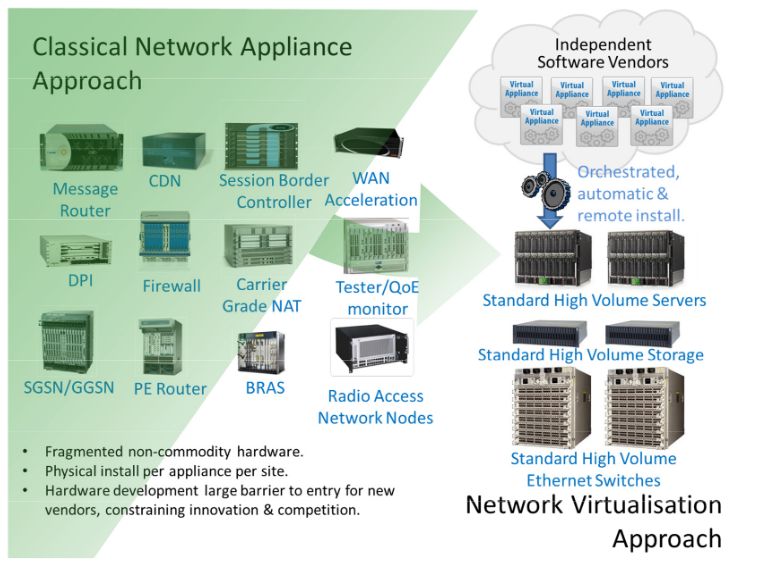
\includegraphics[width=0.55\textwidth]{img/classic_network_vs_nfv.png}
			\label{imagen comparativa classic network nfv}
			\caption{Comparativa enfoque clásico de las redes contra el enfoque virtualizado. [\ref{img: nfv vs classic}]}
		\end{center}
	\end{figure}

	\pagebreak
	
	\noindent La actualidad es cada dispositivo, corresponde con un aparato físico. Son aparatos embebidos y solo cumplen una función específica. Utilizando la virtualización de red, podemos llegar al punto de tenerlo todo virtualizado. Tenemos una 'imagen' de router que la podemos desplegar en cualquier ordenador de caracter general, y cumplir diferentes funciones a la vez (que un router sea a la vez un firewall, por ejemplo).\\
	
	\noindent Las funciones de red están basadas en tener un software y hardware específico para cada dispositivo. NFV nos aporta que esos recursos software y hardware, se despliegan en servidores físicos de proposito general. Por lo tanto, un mismo nodo físico, puede ser DHCP, router o Firewall. [\ref{bib: what is nfv}]\\
	
	\begin{figure}[h!]
		\begin{center}
			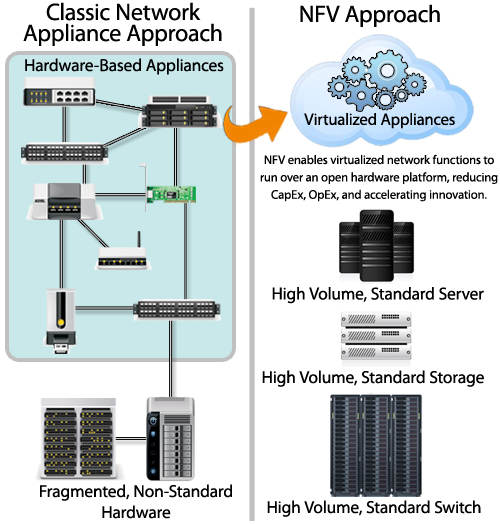
\includegraphics[width=0.4\textwidth]{img/NFV-image-v2.jpg}
			\label{img: comparativa redes classic vs nfv}
			\caption{Comparativa redes clásicas vs redes basadas en NFV [\ref{img: nfv vs classic 2}]}
		\end{center}
	\end{figure}

	\noindent La virtualización de funciones de red supone una manera para reducir costes y acelerar el desarrollo de servicios para los operadores de red a costa de desacoplar funciones como pueden ser un ``firewall'' en un hardware dedicado, moviendolos a servidores virtuales. Tal y como podemos ver en la comparativa de la Figura \ref{img: comparativa redes classic vs nfv}, sustituimos electrónica de red específica, como podrían ser router, switches, etc; por máquinas virtualizadas que se despliegan en servidores de carácter general, dando lugar a un mayor control y escalabilidad de los sistemas físicos. A consecuencia de esto, podemos ver como las redes toman un camino diferente, dejando a atrás el hardware y software propietario, para centrarse en un enfoque basado en el software. \\
	
	\pagebreak
	
\	\subsection{Tecnologías implicadas}
	\noindent Para que este cambio de paradigma se materialice, es decir, pase de ser ``papers'' con soluciones generalistas, y que de verdad estas se materialicen en una solución viable, tienen que realizarse una serie de desarrollos, los cuales provocan que aún a día de hoy sean soluciones experimentales, que aunque son utilizadas en entornos reales, todavía están en continuo desarrollo. Además, aunque estamos hablando de NFV, hay una tecnología extra que también aparece en la ecuación, esta tecnología es el SDN (\textit{Software Defined Networks}). En este caso particular, nos encontramos con que el NFV no puede existir sin el SDN, y viceversa [\ref{bib: sdn y nfv}]. Si tuviéramos que definir brevemente cada una de dichas tecnologías, podríamos resumirlo en lo siguiente:
	\begin{itemize}
		\item \textit{Software Defined Networks}. Suponen un punto de vista de las redes, en las que las propias redes utilizan una serie de controladores, basados en software o en API de control, con el fin de dirigir el tráfico de red y comunicarse con la infraestructura hardware de capas superiores. (ver Figura \ref{img: sdn + nfv})
		 
		\item \textit{Network Functions Virtualizations}. NFV desacopla las funciones de la red de dispositivos de hardware dedicados y las traslada a servidores virtuales, y así se consolidan múltiples funciones en un único servidor físico. Dentro de este servidor físico, podemos distinguir diferentes funciones de red virtuales (VNF), dichas funciones suponen un conjunto de máquinas interconectadas entre sí, y cada una de ellas tiene una función distinta, y además, el conjunto de ellas tienen por objetivo realizar una función que antes era realizada por un equipo físico determinado (un router, firewall o similar). (ver Figura \ref{img: sdn + nfv})
	\end{itemize}

	\begin{figure}[h!]
		\begin{center}
			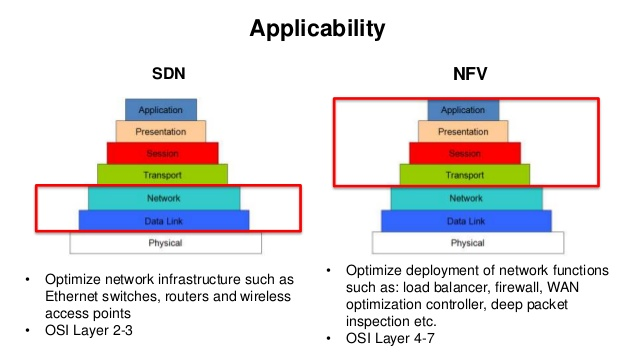
\includegraphics[width=0.8\textwidth]{img/sdn-y-nfv.jpg}
			\caption{Comparativa en capas OSI de las tecnologías NFV y SDN [\ref{img: sdn vs nfv osi}] }
			\label{img: sdn + nfv}
		\end{center}
	\end{figure}

	\pagebreak
	
	\subsection{Virtualización ligera}
	\label{sect: virt ligera}
	
	\noindent Entendemos la virtualización ligera como un tipo de virtualización de un sistema. Dicha virtualización se hace a nivel de sistema operativo, aportando que existan diferentes espacios de usuarios aislados entre sí, sin embargo, a diferencia del concepto `\textit{máquina virtual}' (virtualización dura), en la virtualización ligera todos los sistemas virtualizados dependen del \texttt{kernel} de la máquina host, mientras que en el caso de una máquina virtual, cada instancia tendría su propio \texttt{kernel} (ver Figura \ref{img: virtualization comparative}). [\ref{bib: virt ligera}]\\
	
	\noindent Por lo tanto, las ventajas destacables sobre la virtualización ligera frente a la virtualización ligera serían:
	\begin{itemize}
		\item Un único \texttt{kernel} para todas las instancias que queramos ejecutar.
		\item Eliminamos el correspondiente \textit{overhead} al no tener que emular un \texttt{kernel} para cada instancia.
		\item Menor consumo de CPU y RAM, comparado con las virtualizaciones duras.
		\item Disponen de la posibilidad de iniciar, mover, parar o borrar la instancia virtualizada.
	\end{itemize}
	
	\begin{figure}[h!]
		\begin{center}
			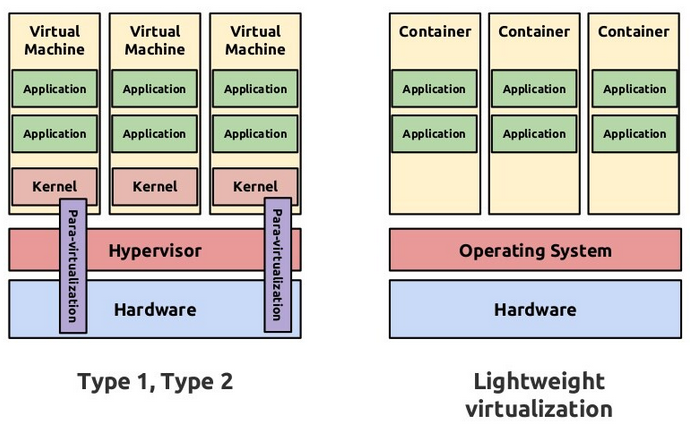
\includegraphics[width=0.8\textwidth]{img/virtualization_comparative.png}
			\caption{Comparativa entre virtualización ligera y virtualización dura [\ref{bib_img: comparativa virt}] }
			\label{img: virtualization comparative}
		\end{center}
	\end{figure}
	
	% Introducción a los siguientes capítulos
	\noindent En consecuencia de tener que utilizar un mismo \texttt{kernel} para todas las instancias, tenemos que profundizar sobre los conceptos de interfaces de red virtuales [\ref{sect: interfaces virtuales}] y espacios de nombres [\ref{sect: espacio nombres}], ya que serán piezas clave para tener nuestras instancias aisladas entre sí, pero a su vez conectadas con los diferentes recursos en red que nosotros definamos.
	
	\pagebreak
	
	\section{Interfaces de red virtuales en \textit{Linux}}
	\label{sect: interfaces virtuales}
	\noindent En este capítulo, vamos a profundizar en el concepto de interfaces de red virtuales, pero las específicas al sistema operativo basados en el kernel de Linux. Hacemos esto ya que los servidores utilizados a gran escala, la mayoría hacen uso de distribuciones de Linux. \\ % TODO
	
	\noindent Linux dispone de una selección muy diferente de interfaces de red que nos permiten, de manera sencilla, el uso de máquinas virtuales o contenedores. En este apartado vamos a mencionar las interfaces más relevantes de cara a la virtualización ligera que proponemos para el despliegue de una red virtualizada. Para obtener una lista completa de las interfaces disponibles, podemos ejecutar el siguiente comando \texttt{ip link help}.\\
	
	\par \noindent En este trabajo, vamos a comentar la siguientes interfaces [\ref{bib:virtual interface list}]:
	\begin{itemize}
		\item MAC compartida: eth0:\{0,1,2...\}
		\item VLAN 802.1q: eth0.\{0,1,2...\}
		\item VLAN 802.1ad: eth0.\{0,1,2...\}.\{0,1,2...\}
		\item Pares de ethernet virtuales (\textit{veth pairs})
		\item TUN/TAP
	\end{itemize}


	\subsection{Nombres predecibles en dispositivos físicos.}
	%\noindent \% Comentar udev (dinamic device management) \% \\
	\noindent Con el fin de comprender como se nombran las diferentes interfaces de red, es necesario que estudiemos el servicio \texttt{udev} (\textit{Dynamic device management}). \texttt{udev} es el gestor de dispositivos que utiliza el kernel de Linux, su función principal es permitir al administrador del sistema operativo registrar manejadores del espacio de usuario para eventos del sistema. Estos eventos que recibe el servicio \texttt{udev} son principalmente generados por el kernel, en respuesta a eventos físicos relacionados con dispositivos periféricos. Por lo tanto, el propósito de \texttt{udev} es actuar sobre la detección de periféricos y con conexiones tipo \textit{hotplug}, pudiendo encadenar acciones necesarias que devuelven el control al kernel, como por ejemplo, cargar módulos específicos o un firmware de un dispositivo. [\ref{bib: udev archwiki}] \\
	
	\noindent Además, \texttt{udev} también se encarga de gestionar los nodos de dispositivos en el directorio \texttt{/dev} añadiendo, enlazando simbólicamente y renombrándolos. Por otro lado, una consideración a tener en cuenta es que \texttt{udev} maneja los eventos de manera concurrente, lo que aporta una mejora de rendimiento, pero a la vez puede dar problemas a la hora de que el orden de carga de los módulos del kernel no se conserva entre los arranques. Un ejemplo de esto podría ser que en el caso de tener dos discos duros (uno llamado \texttt{/dev/sda} y otro \texttt{/dev/sdb}), en el siguiente arranque el orden de de arranque puede variar, generando que ambos identificadores se intercambien entre sí, desencadenando una serie de problemas en nuestro sistema. [\ref{bib: udev archwiki}]\\
	
	\pagebreak
	
	% Captura de regla udev modificada por usuario
	\noindent A modo de ejemplo, el usuario puede crear sus propias reglas, de modo que puede realizar las acciones que ya hemos comentado, de acuerdo a sus propias necesidades. A modo de ejemplo, podemos ver en la siguiente captura (Figura \ref{img: udev rule}) como hemos creado un archivo en la ruta \texttt{/etc/udev/rules.d/} en el que definimos la regla para un dispositivo físico en específico (en este caso un USB). Identificamos el dispositivo que queremos a través de los atributos \texttt{idVendor} e \texttt{idProduct} (atributos necesarios para cualquier dispositivo USB), después le asignamos un "MODE" que corresponde con los permisos que le queremos asignar al dispositivo (en modo numérico) y el grupo al que permitimos acceder al dispositivo.\\
	
	\begin{figure}[h!]
		\begin{center}
			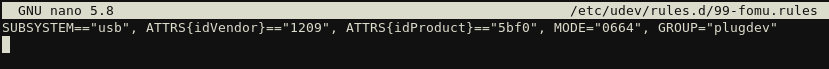
\includegraphics[width=1\textwidth]{img/udev_rule.png}
			\caption{Regla \texttt{udev} definida por el usuario} 
			\label{img: udev rule}
		\end{center}
	\end{figure}
	
	% Comentamos el cambio en el nombrado de las interfaces de red 
	\noindent En el caso de las interfaces físicas de red, vamos a suponer que estamos utilizando el nombrado de interfaces de red antiguo. Esto proviene de que en la últimas versiones del kernel, se ha cambiado la forma en la que las interfaces de red son nombradas por Linux (\texttt{systemd networkd v197} [\ref{bib: systemd networkd v197}]). Es por esto por lo que antes podíamos tener interfaces tal que \texttt{eth0} y ahora nos encontramos con la siguiente nomenclatura \texttt{enps30}. Este cambio surge ya que anteriormente se nombraban las diferentes interfaces conforme el propio ordenador estaba en la etapa de \texttt{boot}, por lo que podría pasar que a lo que nosotros entendíamos como \texttt{eth1}, en el próximo arranque fuera \texttt{eth0}, dando lugar a incontables errores en el sistema. Es por esto por lo que se empecó a trabajar en soluciones alternativas. Por ejemplo, la que acabamos de comentar, utiliza la información aportada por la BIOS del dispositivo para catalogarlo en diferentes categorías, con su formato de nombre para cada categorías. Dichas clasificación corresponde con las siguientes:
	\begin{enumerate}
		\item Nombres incorporados en Firmware/BIOS que proporcionan un número asociado a dispositivos en la placa base. (ejemplo: \texttt{eno1})
		\item Nombres incorporados en Firmware/BIOS proveniente de una conexión PCI Express hotplug, con número asociado al conector. (ejemplo: \texttt{ens1})
		\item Nombres que incorporan una localización física de un conector hardware. (ejemplo: \texttt{enp2s0})
		\item Nombres que incorporan una la MAC de una interfaz. (ejemplo: \texttt{enx78e7d1ea46da})
		\item Sistema clásico e impredecible, asignación de nombres nativa del kernel. (ejemplo: \texttt{eth0})
	\end{enumerate}
	
	\pagebreak
	
	\subsection{MAC compartida \texttt{enp2s0:\{0,1,2...\}}}
	\par \noindent Todas las interfaces asociadas comparten la misma dirección MAC. Cada una de ellas, recibe el nombre de \textit{aliases}. La funcionalidad principal que tienen este tipo de interfaces es la de asignar varias direcciones de IP a una misma interfaz de red.
	
	\begin{verbatim}
$ ip addr add 192.168.56.151/24 broadcast 192.168.56.255 dev enp2s0 
label enp2s0:1
	\end{verbatim}

	\par \noindent Sin embargo, el comando \texttt{iproute2} admite esta misma funcionalidad sin tener que crear interfaces de red extra. Para ello, solo tenemos que asociar cada IP con la interfaz de red deseada.
	\begin{verbatim}
$ ip addr add 192.168.56.151/24 dev enp2s0
$ ip addr add 192.168.56.251/24 dev enp2s0
	\end{verbatim}

	\subsection{VLAN 802.1q \texttt{enp2s0.\{0,1,2...\}}}
	\par \noindent Siguiendo el mismo concepto que la interfaz anterior, pero en este caso utilizando el estándar 802.1q, que permite etiquetar las tramas, para crear una red lógica independiente. Es necesario que la interfaz a la que estemos asignando, sea un puerto trunk, o bien sea tagged para una VLAN específica.
	
	\begin{verbatim}
$ ip link add link enp2s0 name enp2s0.{num} type vlan id {num}
$ ip addr add 192.168.100.1/24 brd 192.168.100.255 dev enp2s0.{num}
$ ip link set dev enp2s0.{num} up
	\end{verbatim}

	\begin{figure}[h!]
		\begin{center}
			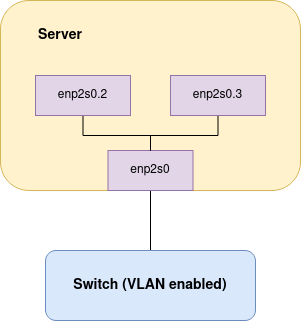
\includegraphics[width=0.4\textwidth]{img/diag_vlan.png}
			\caption{Diagrama conexión VLANs}
		\end{center}
	\end{figure}

	\pagebreak
	
	\subsection{VLAN 802.1ad. \texttt{enp2s0}.\texttt{\{0,1,2...\}.\{0,1,2...\}}}
	\noindent En este aparatado comentamos la interfaz virtual asociada al estándar 802.1ad, dicho estándar supone una actualización respecto a las VLANs basadas en 802.1q, pero añadiendo la posibilidad de tener dos tags dentro de mismo frame ethernet. En el caso del estándar 802.1q, solo podíamos tener un tag. El estándar de vlans 802.1ad es realmente útil cuando el proveedor de red y el usuario de dicha red quieren utilizar VLANs, además que amplía el límite de 4094 VLANs diferentes permitidas por el estándar 802.1Q [\ref{bib: 802.1ad}][\ref{bib: FS QinQ}]. Otra forma de la que nos podemos encontrar esta interfaz es bajo el nombre ``QinQ''. \\
	
	\noindent La estructura de la trama ethernet sigue la siguiente estructura,
	
	\begin{figure}[h]
		\begin{center}
			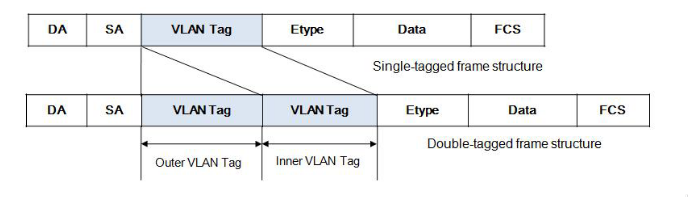
\includegraphics[width=0.8\textwidth]{img/ethernet_8021ad.png}
			\caption{Trama ethernet utilizando VLAN 802.1ad [\ref{img: frame ethernet 802.1ad}]}
			\label{ethernet 802.1ad}
		\end{center}
	\end{figure}
	
	\noindent Para configurar un enlace utilizando este estándar, tenemos que ejecutar los siguientes comandos [\ref{bib: openwrt virtual network interfaces}]:
	\begin{verbatim}
$ ip link add link eth0 eth0.1000 type vlan proto 802.1ad id 1000
$ ip link add link eth0.1000 eth0.1000.1000 type vlan proto 802.1q id 1000
 	\end{verbatim}
 
 	\noindent De esta manera, lo que hacemos es asociar una primera VLAN a una interfaz de red, utilizando 802.1ad, después a esa misma interfaz con identificador, podemos asignar otra nueva VLAN, pero esta vez utilizando el estándar 802.1q. Por lo tanto, al final nos quedaría una interfaz similar a \texttt{eth0.1000.1000} en la que podemos distinguir dos identificadores de red virtual.
	
	\pagebreak
	
	\subsection{Pares VETH.}
	\noindent Los \texttt{veth} (Ethernet virtuales) son un dispositivo virtual que forman un túnel local ethernet. El dispositivo se crea en parejas. [\ref{bib:virtual interface list}]\\
	
	\noindent Los paquetes transmitidos por un extremo del ethernet virtual se reciben inmediatamente en el otro extremo. Si alguno de ellos se encuentra apagado, decimos que el link de la pareja esta también apagado. A modo de ejemplo, nos fijamos una estructura básica en la que dos aplicaciones se comunican utilizando \texttt{veth}, tal y como vemos en la figura (\ref{ej1 veth})\\
	
	\begin{figure}[h]
		\begin{center}
			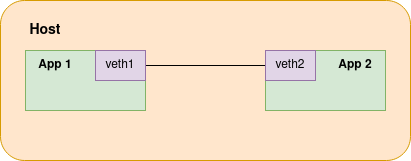
\includegraphics[width=0.5\textwidth]{img/veth_ej1.png}
			\caption{Ejemplo básico de utilización de pares virtuales ethernet}
			\label{ej1 veth}
		\end{center}
	\end{figure}

	\noindent Las interfaces virtuales ethernet se inventaron con el fin de comunicar diferentes \textit{network namespaces}. Aunque profundizaremos en ello más adelante, los \texttt{namespace} de Linux permiten encapsular recursos globales del sistema de forma aislada, evitando que puedan interferir con procesos que estén fuera del \texttt{namespace}.\\
	
	\noindent La configuración necesaria para implementar el ejemplo de la figura \ref{ej1 veth} sería el siguiente [\ref{bib:example netns veth}]:
	
	\begin{verbatim}
$ ip netns add app1
$ ip netns add app2
$ ip link add veth1 netns app1 type veth peer name veth2 netns app2
	\end{verbatim}
	
	\noindent De esta manera, tendríamos creados los \texttt{namespaces} \texttt{app1} y \texttt{app2}, que estarían interconectados entre sí. Ahora procedemos a asignar una IP a cada interfaz. 
	
	\begin{verbatim}
$ ip netns exec app1 ip addr add 10.1.1.1/24 dev veth1
$ ip netns exec app1 ip link set veth1 up
$ ip netns exec app2 ip addr add 10.1.1.2/24 dev veth2
$ ip netns exec app2 ip link set veth2 up
	\end{verbatim}
	
	\pagebreak

	\noindent Para comprobar que hay conectividad entre las diferentes aplicaciones (\texttt{app1} y \texttt{app2}) utilizamos la función del comando \texttt{ip} para ejecutar programas dentro de un \texttt{network namespace}, en este caso realizar un ping entre ambas aplicaciones:
	
	\begin{verbatim}
$ ip netns exec app1 ping 10.1.1.2
	\end{verbatim}
	
	\noindent Por otro lado, si quisiéramos una topología más compleja, como por ejemplo que varios \texttt{namespaces} puedan hacer uso de una interfaz física, tendríamos que añadir un elemento extra a nuestro sistema. El diagrama de la topología podría ser tal que así:
	
	\begin{figure}[h!]
		\begin{center}
			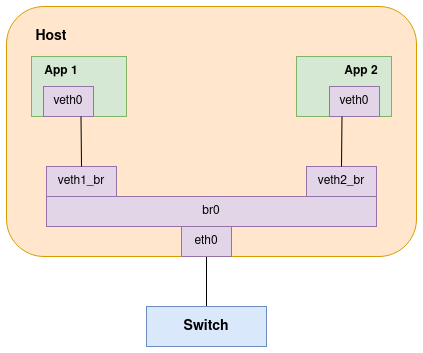
\includegraphics[width=0.5\textwidth]{img/veth_ej2.png}
			\caption{Ejemplo avanzado de utilización de pares virtuales ethernet, utilizando \texttt{bridge}}
			\label{ej2 veth}
		\end{center}
	\end{figure}
	
	\noindent Como podemos comprobar en la figura \ref{ej2 veth}, es necesario que utilicemos un ``bridge" para que podamos conectar ambas interfaces virtuales a una interfaz física, para replicar dicha topología, ejecutaremos los siguientes comandos:
	
	\begin{verbatim}
$ ip netns add app1
$ ip netns add app2
$ ip link add veth1_br type veth peer name veth0 netns app1
$ ip link add veth2_br type veth peer name veth0 netns app2

	\end{verbatim}
	
	\noindent Para definir un bridge entre las diferentes interfaces virtuales que hemos creado, utilizaremos una interfaz tipo \textit{bridge} de Linux, o bien podemos configurar dicho \textit{bridge} usando \textit{Open vSwitch}. \textit{Open vSwitch} es un programa de código abierto diseñado para ser utilizado como un switch multi-capa virtual [\ref{bib: open vswitch}][\ref{bib: veth netns ovs}].
	
	\begin{verbatim}
$ ip link add veth1_br type veth peer name veth0 netns app1
$ ip link add veth2_br type veth peer name veth0 netns app2
$ ovs-vsctl add-br ovsbr0
$ ovs-vsctl add-port ovsbr0 veth1_br
$ ovs-vsctl add-port ovsbr0 veth2_br
$ ovs-vsctl add-port ovsbr0 eth0
	\end{verbatim}

	\noindent Por último, añadimos las direcciones IP que nos faltan en la topología:
	
	\begin{verbatim}
$ ip addr add 10.1.1.10/24 dev veth1_br
$ ip link set veth1_br up
$ ip addr add 10.1.1.20/24 dev veth2_br
$ ip link set veth2_br up
$ ip netns exec app1 ip addr add 10.1.1.15/24 dev veth0
$ ip netns exec app1 ip link set veth0 up
$ ip netns exec app2 ip addr add 10.1.1.25/24 dev veth0
$ ip netns exec app2 ip link set veth0 up
$ ip netns exec app1 ip link set lo up
$ ip netns exec app2 ip link set lo up
	\end{verbatim}

	\noindent De esta manera, ya tendríamos la topología configurada con conectividad entre las diferentes aplicaciones, además de cada aplicación con una interfaz física de la máquina, todo esto utilizando una interfaz tipo \texttt{bridge}.

	\subsection{TUN/TAP}
	\noindent TUN/TAP son dos interfaces de red virtuales de Linux, que permiten dar conectividad entre programas dentro del espacio de usuario, es decir permiten conectar aplicaciones en específico con el kernel. Esta interfaz es expuesta al usuario mediante la ruta \texttt{/dev/net/tun}. Como bien hemos mencionado, existen dos tipos de interfaces virtuales controladas por \texttt{/dev/net/tun}: 
	
	\begin{itemize}
		\item TUN. Interfaces encargadas de transportar paquetes IP (trabaja sobre la capa 3).
		\item TAP. Interfaces encargadas de transportar paquetes Ethernet (trabaja sobre la capa 2).
	\end{itemize}
	
	\vspace{5px}

	\noindent \textbf{\large TUN (Capa 3)}\\
	\noindent Las interfaces TUN (\texttt{IFF\_TUN}) transportan paquetes PDU (\textit{Protocol Data Units}) de la capa 3 [\ref{bib: tun vs tap}]:
	\begin{itemize}
		\item En la práctica, transporta paquetes IPv4 y/o paquetes IPv6.
		\item La función \texttt{read()} devuelve un paquete de capa 3 PDU, es decir un paquete IP.
		\item Utilizando la función \texttt{write()} podemos enviar un paquete IP.
		\item No hay capa 2 en esta interfaz, por lo que los mecanismos que se ejecutan en esta capa no estarán presentes en la comunicación. Por ejemplo, no tenemos ARP.
		\item Pueden funcionar como interfaces tipo \textit{Point to Point}.
	\end{itemize}
	
	\pagebreak
	
	\noindent \textbf{\large TAP (Capa 2)}\\
	\noindent Las interfaces TAP (\texttt{IFF\_TAP}) transportan paquetes de capa 2 \ref{bib: tun vs tap}: 
	\begin{itemize}
		\item En la práctica, transporta \textit{frames Ethernet}, por lo tanto, actuaría como si fuera un adaptador virtual de Ethernet (``bridge virtual'').
		\item La función \texttt{read()} devuelve un paquete de capa L2, un \textit{frame Ethernet}.
		\item Utilizando la función \texttt{write()} permite enviar un \textit{frame Ethernet}.
		\item Podemos cambiar la MAC asociada a nuestra interfaz TAP utilizando el parámetro \texttt{SIOCSIFHWADDR}, en la función \texttt{ioctl()}, la cual usamos para crear un TUN/TAP dentro de nuestra aplicación.
	\end{itemize}

	\vspace{5px}

	% Imagen comparativa entre TUN/TAP
	\begin{figure}[h!]
		\begin{center}
			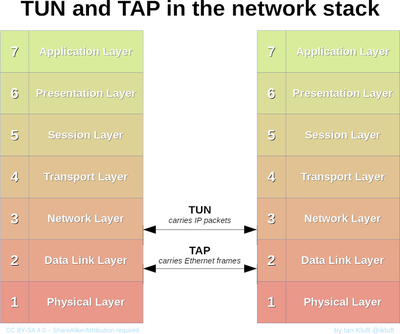
\includegraphics[width=0.6\textwidth]{img/tun_vs_tap.png}
			\caption{Comparativa en capa OSI de las interfaces TUN/TAP. [\ref{bib_img: tun tap}]}
			\label{img: tun vs tap}
		\end{center}
	\end{figure}
	
	\noindent Si nos fijamos en la figura \ref{img: tun vs tap}, podemos ver las diferencias entre ambas interfaces. Aún así, hay una que se utiliza mucho más que la otra, esta interfaz es TAP. Las interfaces tipo TAP son muy ampliamente utilizadas para realizar ``túneles virtuales'' para una aplicación en concreto. Sería la propia aplicación la encargada de monitorizar dicho ``túnel''. Podemos encontrar aplicaciones TAP en hipervisores o en clientes VPN.
	
	\pagebreak
	
	\noindent En el caso de que queramos crear interfaces TUN/TAP fuera de una aplicación, es decir, desde la línea de comandos, tendremos que utilizar los programas \texttt{tunctl} o \texttt{ip}. Para ello, podemos revisar los ejemplos \ref{lst: ej1 tunctl} y \ref{lst: ej2 tuntap ip} donde se comentan algunos de los comandos más importantes para trabajar con estar interfaces en cada uno de los programas mencionados.
	
	\vspace{10px}
	
	% Ejemplo 1: Creacion de tun/tap utilizando la linea de comandos
	\begin{lstlisting}[language=Bash, label=lst: ej1 tunctl, caption=Ejemplo de uso de \texttt{tunctl} para controlar interfaces TUN/TAP [\ref{bib: tunctl + ip}]]
# Create the tap interface by default
tunctl 
# equivalent to
tunctl -p

# For users 'user' create a tap interface
tunctl -u user

# Create  Tun interface
tunctl -n
# Configure IP Address for interface and enable
ip addr add 192.168.0.254/24 dev tap0
ip link set tap0 up
# Add routing to interface
ip route add 192.168.0.1 dev tap0

# Delete interface
tunctl -d tap0
	\end{lstlisting}

	\vspace{10px}

	% Ejemplo 1.1: Creacion tun/tap pero usando comando ip
	\begin{lstlisting}[language=Bash, label=lst: ej2 tuntap ip, caption=Ejemplo de uso de \texttt{ip} para controlar interfaces TUN/TAP [\ref{bib: tunctl + ip}]]
# Show help
ip tuntap help

# Create tun/tap devices
ip tuntap add dev tap0 mod tap		# create tap
ip tuntap add dev tun0 mod tun		# create tun

# Delete tun/tap devices
ip tuntap del dev tap0 mod tap		# delete tap
ip tuntap del dev tun0 mod tun		# delete tun
	\end{lstlisting}

	\pagebreak
	
	\noindent \textbf{\large Ejemplo de aplicación que crea una interfaz tuntap}\\

	\noindent Por otro lado, otra manera de trabajar con estas interfaces, es dejar que el programa que estemos utilizando cree dichas interfaces. Es por esto por lo que dentro del programa podemos definir que se refiera a la ruta \texttt{/dev/net/tun} para crear la interfaz necesaria. A modo de ejemplo, se implementa un programa en C que crea una interfaz TUN/TAP (en el programa elegimos cual de las dos queremos) y que devuelve el tamaño de los paquetes que reciba en dicha interfaz. Este ejemplo nos sirve para comprobar con una aplicación puede crear y gestionar una interfaz, y además, mediante un programa externo de captura de paquetes (\texttt{Wireshark}, \texttt{tcpdump}, etc...) ver los paquetes que llegan a la interfaz y cual es su estructura. \\
	
	\noindent El código utilizado sería el que vemos en [\ref{lst:tuntap.c}]. Es importante comentar que en la linea 80 podemos modificar el tipo de interfaz que vamos a crear, usaremos \texttt{IFF\_TUN} para crear un TUN y \texttt{IFF\_TAP} para crear un TAP.
	% Ejemplo: 2 Apps en C que se comunican utilizan TAP
	\vspace{10px}
	\begin{lstlisting}[language=C, label=lst:tuntap.c, caption=Aplicación de ejemplo para crear tun/tap (tuntap.c) [\ref{bib: code tuntap.c}]]
/**
Receive incoming packages over tun/tap device. 
stdout -> size of received package
**/

#include <net/if.h>
#include <sys/ioctl.h>
#include <sys/stat.h>
#include <fcntl.h>
#include <string.h>
#include <sys/types.h>
#include <linux/if_tun.h>
#include <stdlib.h>
#include <stdio.h>

int tun_alloc(int flags)
{
	
	struct ifreq ifr;
	int fd, err;
	char *clonedev = "/dev/net/tun";
	
	if ((fd = open(clonedev, O_RDWR)) < 0) {
		return fd;
	}
	
	memset(&ifr, 0, sizeof(ifr));
	ifr.ifr_flags = flags;
	
	if ((err = ioctl(fd, TUNSETIFF, (void *) &ifr)) < 0) {
		close(fd);
		return err;
	}
	
	printf("Open tun/tap device: %s for reading...\n", ifr.ifr_name);
	
	return fd;
}

int main()
{
	
	int tun_fd, nread;
	char buffer[1500];
	
	/* Flags: IFF_TUN   - TUN device (no Ethernet headers)
	*        IFF_TAP   - TAP device
	*        IFF_NO_PI - Do not provide packet information
	*/
	tun_fd = tun_alloc(IFF_TAP | IFF_NO_PI);
	
	if (tun_fd < 0) {
		perror("Allocating interface");
		exit(1);
	}
	
	while (1) {
		nread = read(tun_fd, buffer, sizeof(buffer));
		if (nread < 0) {
			perror("Reading from interface");
			close(tun_fd);
			exit(1);
		}
		
		printf("Read %d bytes from tun/tap device\n", nread);
	}
	return 0;
}
	\end{lstlisting}

	\pagebreak

	\noindent Los pasos para realizar este ejemplo serían los siguientes:
	\begin{lstlisting}[language=Bash, label=lst: instr tuntap.c , caption=Instrucciones para realizar las pruebas con el código [\ref{lst:tuntap.c}]]
# Guardamos el codigo anterior en tuntap.c
# Compilamos el programa
gcc tuntap.c -o tun

### Terminal 1
# Ejecutamos el binario, este se quedara a la escucha en la interfaz creada
./tun

### Terminal 2
# Asignamos una IP a la interfaz recien creada
ip addr add 192.168.209.138/24 dev tun0
ip link set dev tun0 up

# Capturamos el trafico que viaja por la interfaz
tcpdump -i tun0

### Terminal 3
# Mandamos trafico a la interfaz creada, un ping por ejemplo:
ping -c 4 192.168.209.139 -I tun0
	\end{lstlisting}
	
	\pagebreak
	
	%\vspace{10px}
	\noindent \textbf{\large Ejemplo aislamiento entre puertos usando interfaz tuntap}\\
	
	\noindent En este ejemplo, queremos comprobar el funcionamiento de una interfaz \texttt{tap}, pero poniéndonos en el caso de que el usuario cree dicha interfaz mediante el comando \texttt{ip} y un programa externo se asocie a dicha interfaz. Para ello, vamos a utilizar la aplicación \texttt{sock} [\ref{bib: sock}], que nos servirá para crear un socket IP en un puerto específico.
	
	\begin{lstlisting}[language=Bash, caption={Compilar e instalar programa \texttt{sock} (\ref{bib: sock})}]
mkdir ~/tmp
cd tmp
tar zxvf sock-0.3.2.tar.gz
cd sock-0.3.2
./configure
make
sudo make install
	\end{lstlisting}

	\noindent Una vez tenemos el programa instalado, podemos proceder a crear la interfaz \texttt{tap}.
	
	\begin{lstlisting}[language=Bash, caption={Creación interfaz TAP}]
ip tuntap add dev tap0 mode tap
ip address add 192.168.3.1/24 dev tap0
ip link set tap0 up
ip route add 192.168.3.1 dev tap0
	\end{lstlisting}

	%\pagebreak
	
	\noindent Una vez ya tenemos creada la interfaz, podemos proceder a comprobar la funcionalidad utilizando el programa \texttt{sock}. Para ello, vamos a crear dos instancias cliente-servidor, cada una con un puerto asociado diferente.
	
	\begin{lstlisting}[language=Bash, caption={Uso de aplicacion \texttt{sock} para crear cliente servidor asociado a un puerto}]
sock -s 192.168.3.1 1025    # Terminal 1 (servidor)
sock 192.168.3.1 1025       # Terminal 2 (cliente)

sock -s 192.168.3.1 1026    # Terminal 3 (servidor)
sock 192.168.3.1 1026       # Terminal 4 (cliente)
	\end{lstlisting}

	\pagebreak

	\noindent De esta manera, podemos escribir en cada una de las terminales, y comprobar que solo son recibidas por el servidor, o cliente, asociado al puerto de la terminal en cuestión. Es decir, en las interfaces \texttt{tuntap} tenemos aislamiento entre los diferentes puertos, por lo que funcionan de manera equivalente a un enlace \texttt{ethernet} físico. En la figura (\ref{img: ejemplo sock}) podemos ver el ejemplo realizado.
	
	\begin{figure}[h!]
		\begin{center}
			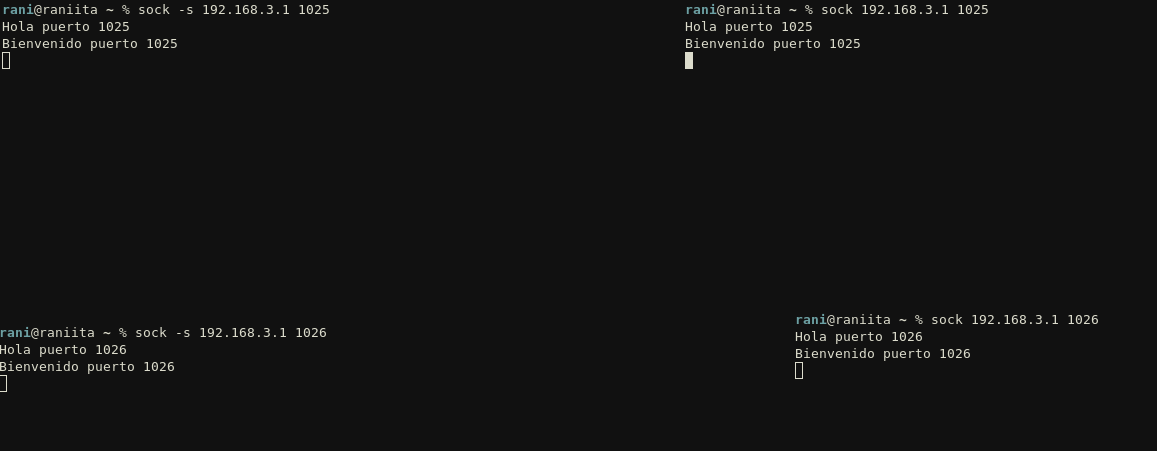
\includegraphics[width=1\textwidth]{img/ejemplo_sock.png}
			\caption{Uso de la aplicación \texttt{sock} con interfaces \texttt{tuntap}.}
			\label{img: ejemplo sock}
		\end{center}
	\end{figure}
	
	\noindent Si comprobamos la tabla de enrutamiento de la interfaz creada, \texttt{tap0}, podemos ver como aparece asociado el trafico de la IP que le dimos a dicha interfaz, con que utilice la interfaz \texttt{tap0}. (Ver figura [\ref{img: ip route tap}])
	
	\begin{figure}[h!]
		\begin{center}
			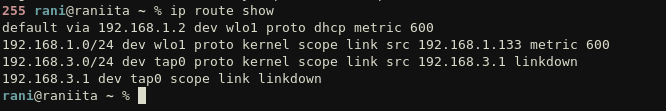
\includegraphics[width=0.75\textwidth]{img/tabla_encaminamiento_tuntap.png}
			\caption{Tabla de encamientamiento para una interfaz tuntap.}
			\label{img: ip route tap}
		\end{center}
	\end{figure}

	\pagebreak
	
	\noindent Por último, podemos comprobar la estructura de los paquetes enviados utilizando programas como \texttt{Wireshark}, \texttt{tcpdump}, etc. Es importante comentar que aunque los paquetes deberían viajar por la interfaz \texttt{tap0}, el kernel los redirige por \texttt{loopback}. En la figura \ref{img: wireshark tuntap} podemos ver un ejemplo de captura de un paquete enviado por el \texttt{tap0}.
	
	\begin{figure}[h!]
		\begin{center}
			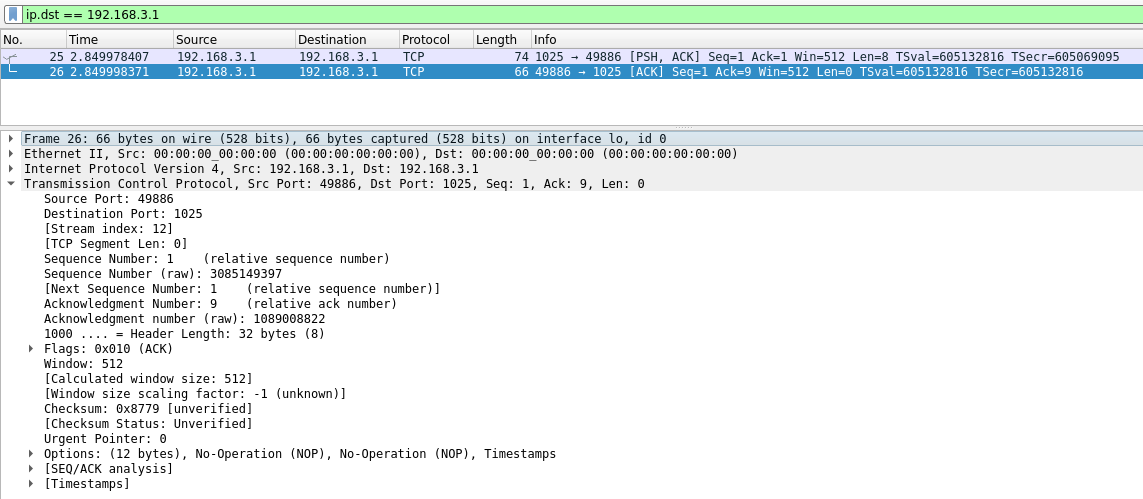
\includegraphics[width=1\textwidth]{img/wireshark_tuntap.png}
			\caption{Captura de un paquete emitido por la interfaz \texttt{tap0}.}
			\label{img: wireshark tuntap}
		\end{center}
	\end{figure}
	
	
	\pagebreak
	\section{Espacio de nombres en \textit{Linux}}
	\label{sect: espacio nombres}
	\subsection{¿Qué es un \textit{espacio de nombres}?}
	\noindent Los \textit{espacios de nombres}, o también llamados, \textit{namespaces}, son una característica del kernel de Linux que permite gestionar los recursos del kernel, pudiendo limitarlos a un proceso o grupo de procesos. Suponen una base de tecnología que aparece en las técnicas de virtualización más modernas (como puede ser Docker, Kubernetes, etc). A un nivel alto, permiten aislar procesos respecto al resto del kernel. \\
	
	\par \noindent El objetivo de cada \textit{namespaces} es adquirir una característica global del sistema como una abstracción que haga parecer a los procesos de dentro del \textit{namespace} que tienen su propia instancia aislada del recurso global.
	
	% TODO
	\subsection{¿Cómo crear/acceder a un \textit{namespace}?}
	\noindent Los namespaces normalmente se suelen asociar a procesos o aplicaciones en específico. Para manipular estos namespaces, podemos destacar las siguientes herramientas: 
	\begin{itemize}
		\item \texttt{unshare}. Permite asociar un namespace a un archivo. Si habia un namespace ya en ese archivo, lo sobreescribe. No nos permite reutilizar un namespace.
		\item \texttt{nsenter}. Puede acceder al namespace de un archivo existente. Podemos asociar el namespace a un archivo del sistema, de modo que aunque cerremos el proceso asociado, el archivo sigue existiendo, y por lo tanto puede ser reutilizado.
	\end{itemize}

	\noindent En resumen, si quisieramos mantener ``vivo'' un namespace, sería necesario que lo asociemos con un archivo del sistema, y después volver a ``crear'' el namespace con la herramienta \texttt{nsenter} apuntando a dicho archivo. A modo de ejemplo, sería tal que así:
	
	\begin{lstlisting}[language=Bash, label=lst: persistencia ns, caption=Ejemplo de un persistencia namespace]
touch /root/ns-uts											# Creamos un archivo
unshare --uts=/root/ns-uts /bin/bash		# Asociamos namespace UTS al archivo
hostname FooBar

# Salimos del namespace
exit

# Volvemos a entrar al namespace
nsenter --uts=/root/ns-uts /bin/bash
hostname                  # Nos devuelve 'FooBar'

# Salimos del namespace
exit

umount /root/ns-uts 			# Eliminamos el namespace definitivamente
	\end{lstlisting}
	
	\vspace{10px}
	
	\noindent Tal y como vemos en el ejemplo (\ref{lst: persistencia ns}), utilizamos los comandos \texttt{unshare} y \texttt{nsenter} para manipular un namespace de tipo UTS (hostname), veremos más en profundidad este namespace en el apartado \ref{sect: uts namespace}. Lo importante es comprobar que si asociamos un namespace a un archivo, podemos recuperar dicho namespace si utilizamos el comando \texttt{nsenter}. Además, si quisieramos eliminar permanentemente dicho namespace, tendríamos que hacer uso del comando \texttt{umount}.
	
	\subsection{¿Cúantos \textit{namespaces} hay?}
	\par\noindent El kernel ha estado en contaste evolución desde que 1991, cuando Linus Torvalds comenzó el proyecto, actualmente sigue muy activo y se siguen añadiendo nuevas características. El origen de los namespaces se remonta a la versión del kernel 2.4.19, lanzada en 2002. Conforme fueron pasando los años, más tipos diferentes de namespaces se fueron añadiendo a Linux. El concepto de \textit{User namespaces}, se consideró terminado con la versión 3.9. [\ref{bib:ns overview}]\\
	\par \noindent Actualmente, tenemos 8 tipos diferentes de namespaces, siendo el último añadido en la versión 5.8 (lanzada el 2 de Agosto de 2020). 
	
	\begin{enumerate}
		\item UTS (hostname)
		\item Mount (mnt)
		\item Process ID (pid)
		\item Network (net)
		\item User ID (user) 
		\item Interprocess Communication (ipc)
		\item Control group (cgroup)
		\item Time [\ref{bib:time ns}]
	\end{enumerate}
	
	\pagebreak
	
	\subsubsection{UTS namespace}
	\label{sect: uts namespace}
	\par \noindent El tipo más sencillo de todos los namespaces. La funcionalidad consiste en controlar el hostname asociado del ordenador, en este caso, del proceso o procesos asignados al namespace. Existen tres diferentes rutinas que nos permiten obtener y modifcar el hostname: 
	\begin{itemize}
		\item \textit{sethostname()}
		\item \textit{setdomainname()}
		\item \textit{uname()}
	\end{itemize}
	En una situación normal sin namespaces, se modificaría una String global, sin embargo, si estamos dentro de un namespace, los procesos asociados tienen su propia variable global asignada.\\
	
	% example uts: https://medium.com/@teddyking/linux-namespaces-850489d3ccf
	% https://www.cloudsavvyit.com/742/what-are-linux-namespaces-and-what-are-they-used-for/
	\par \noindent Un ejemplo muy basico de uso de este namespaces podría ser el siguiente [\ref{bib:ns tutorial1}]:\\
	\begin{lstlisting}[language=bash, caption=Ejemplo de uso de UTS namespace]
$ sudo su			# super user
$ hostname			# current hostname
> arch-linux					
$ unshare -u /bin/sh		# shell with UTS namespace
$ hostname new-hostname		# set hostname
$ hostname			# check hostname of the shell
> new-hostname
$ exit				# exit shell and namespace
$ hostname			# original hostname
> arch-linux
	\end{lstlisting}

	\addvspace{10px}

	\par \noindent En el ejemplo planteado, vemos que utilizamos el comando \texttt{unshare}. Utilizando la documentación de dicho comando, \texttt{man unshare}. Podemos deducir los siguiente:
	\begin{itemize}
		\item Ejecuta un programa con algunos namespaces diferentes del host.
		\item En los parametros podemos especificar cual o cuales namespaces queremos desvincular.
		\item Tenemos que especificar la ruta del ejecutable que queremos aislar
		\item La sintaxis sería tal que: \texttt{unshare [options] <program> [<argument>...]}
	\end{itemize}
	
	\pagebreak
	
	\subsubsection{Mount namespace}
	\par \noindent Un \textit{mount namespace (mnt)} supone otro tipo de espacio de nombres, en este caso relacionado con los \textit{mounts} de nuestro sistema. Lo primero es entender a que nos referimos cuando hablamos de \textit{mount}. \textit{Mount}, o montaje, hace referencia a conectar un sistema de archivos adicional que sea accesible para el sistema de archivos actual de un ordenador. Un \texttt{mount}, tiene asignado lo que se llama \textit{mount point}, que corresponde con el directorio en el que está accesible el sistema de archivo que previamente hemos montado.\\
	
	\par \noindent Por lo tanto, un namespace de tipo \textit{mount} nos permite modificar un sistema de archivos en concreto, sin que el host pueda ver y/o acceder a dicho sistema de archivos. Un ejemplo básico de esta funcionalidad podría ser la siguiente:
	
	\addvspace{10px}
	
	\begin{lstlisting}[language=bash, caption=Example of usage mount namespace]
$ sudo su		# run a shell in a new mount namespace
$ unshare -m /bin/sh
$ mount --bind /usr/bin/ /mnt/
$ ls /mnt/cp
> /mnt/cp
$ exit			# exit the shell and close namespace
$ ls /mnt/cp
> ls: cannot access '/mnt/cp': No such file or directory
	\end{lstlisting}

	\addvspace{10px}
	
	\par \noindent Como vemos en el ejemplo, dentro del namespaces lo que hacemos es crear un \textit{mount} de tipo \textit{bind}, que tiene por función que un archivo de la máquina host se monte en un directorio en específico, en este caso, un directorio unicamente del programa que hemos asignado al namespace. Otro ejemplo de uso de estos namespaces es crear un sistema de archivos temporal que solo sea visible para ese proceso.
	
	% TODO
	% Ejemplo: limitar un USB a que solo lo vea un namespace
	
	\pagebreak
	
	\subsubsection{Process ID namespace}
	\par \noindent Para entender en que consiste este namespace, primero tenemos que conocer la definición de \textit{process id} dentro del Kernel. En este caso, \textit{process id} hace referencia a un número entero que utiliza el Kernel para identificar los procesos de manera unívoca. [\ref{bib:pid wikipedia}]\\
	
	\par \noindent Concretando, aísla el namespace de la ID del proceso asignado, dando lugar a que, por ejemplo, otros namespaces puedan tener el mismo PID. Esto nos lleva a la situación de que un proceso dentro de un \textit{PID namespace} piense que tiene asignado el ID "1", mientras que en la realidad (en la máquina host) tiene otro ID asignado.
	
	\addvspace{10px}
	
	\begin{lstlisting}[language=bash, caption=Uso de process id namespace]
$ echo $$		# PID de la shell
$ ls -l /proc/$$/ns	# ID espacios de nombres 
$ sudo unshare -f --mount-proc -p /bin/sh
$ echo $$		# PID de la shell dentro del ns
$ ls -l /proc/$$/ns	# nuevos ID espacio de nombres
$ ps

$ ps -ef 		# ejecutar en una shell fuera del ns. Comparar PID
$ exit
	\end{lstlisting}

	\addvspace{10px}
	
	\par \noindent Si ejecutamos el ejemplo, lo que podemos comprobar es que el ID del proceso que está dentro del namespaces (\texttt{echo \$\$}), no coincide con el proceso que podemos ver de la máquina host (\texttt{ps -ef | grep /bin/sh}). Más concretamente, el primer proceso creado en un PID namespace recibirá el pid número 1, y además de un tratamiento especial ya que supone  un \texttt{init process} dentro de ese namespace [\ref{bib:ns tutorial1}].
	
	% revisar: https://www.redhat.com/sysadmin/linux-pid-namespaces
	% https://man7.org/linux/man-pages/man7/pid_namespaces.7.html
	
	\pagebreak
	
	\subsubsection{Network namespace (netns)}
	\par \noindent Este namespaces nos permite aislar la parte red de una aplicación o proceso que nosotros elijamos. Con esto conseguimos que el \textit{stack} de red de la máquina host sea diferente al que tenemos en nuestro namespace. Debido a esto, el namespace crea una interfaz virtual, conjunto con el resto de necesidades para conformar un stack de red completo (tabla de enrutamiento, tabla ARP, etc...).\\
	
	\par \noindent Para crear un \textit{namespace} de tipo \textit{network}, y que este sea persistente, utilizamos la \textit{tool} ip (del \textit{package} iproute2).
	\begin{lstlisting}[language=bash, caption=Creation persistent network namespace]
$ ip netns add ns1
	\end{lstlisting}

	\par \noindent Este comando creará un network namespace llamado ns1. Cuando se crea dicho namespace, el comando ip realiza un montaje tipo bind en la ruta /var/run/netns, permitiendo que el namespace sea persistente aún sin tener un proceso asociado.
	\begin{lstlisting}[language=bash, caption=Comprobar network namespaces existentes]
$ ls /var/run/netns
or
$ ip netns
	\end{lstlisting}
	
	\addvspace{10px}

	\par \noindent Como ejemplo, podemos proceder a añadir una interfaz de \textit{loopback} al namespace que previamente hemos creado:
	\begin{lstlisting}[language=bash, caption=Asignar interfaz loopback a un namespace]
$ ip netns exec ns1 ip link dev lo up
$ ip netns exec ns1 ping 127.0.0.1
> PING 127.0.0.1 (127.0.0.1) 56(84) bytes of data. 
> 64 bytes from 127.0.0.1: icmp_seq=1 ttl=64 time=0.115 ms
	\end{lstlisting}

	\par \noindent La primera línea de este ejemplo, corresponde con la directiva que le dice al namespace que "levante" la interfaz de loopback. La segunda línea, vemos como el namespace ns1 ejecuta el ping a la interfaz de loopback (el loopback de ese namespace).
	
	\addvspace{10px}
	
	\par \noindent Es importante mencionar, que aunque existen más comandos para gestionar las redes dentro de linux (como pueden ser ifconfig, route, etc), el comando ip es el considerado sucesor de todos estos, y los anteriores mencionados, dejarán de formar parte de Linux en versiones posteriores. Un detalle a tener en cuenta con el comando ip, es que es necesario tener privilegios de administrador para poder usarlo, por lo que deberemos ser root o utilizar sudo.
	
	\addvspace{10px}
	
	\par \noindent Por lo tanto, utilizando el comando ip, podemos recapitular que si utilizamos la siguiente directiva, podemos ejecutar el comando que nosotros indiquemos, pero dentro del network namespace que previamente hemos creado.
	\begin{lstlisting}[language=bash, caption=Ejecutar cualquier programa con un network namespace]
$ ip netns exec <network-namespace> <command>
	\end{lstlisting}

	\pagebreak
	
	\noindent \textbf{\large Ejemplo práctico}\\
	\par \noindent Una de las problemáticas que supone el uso de los network namespaces, es que solo podemos asignar \textbf{una interfaz real} a \textbf{un namespace}. Suponiendo el caso en el que el usuario root tenga asignada la interfaz eth0 (identificador de una interfaz de red física), significaría que solo los programas en el namespace de root podrán acceder a dicha interfaz. En el caso de que eth0 sea la salida a Internet de nuestro sistema, pues eso conllevaría que no podríamos tener conexión a Internet en nuestros namespaces. La solución para esto reside en los \textbf{veth-pair}.
	
	\addvspace{10px}
	
	\par \noindent Un veth-pair funciona como si fuera un cable físico, es decir, interconecta dos dispositivos, en este caso, interfaces virtuales. Consiste en dos interfaces virtuales, una de ellas asignada al root namespace, y la otra asignada a otro network namespace diferente. Si a esta arquitectura le añadimos una configuración de IP válida y activamos la opción de hacer NAT en el eth0 del host, podemos dar conectividad de Internet al network namespace que hayamos conectado.
	
	\addvspace{10px}
	
	\begin{lstlisting}[language=bash, caption=Ejemplo configuración de NAT entre eth0 y veth]
# Remove namespace if exists
$ ip netns del ns1 &>/dev/null

# Create namespace
$ ip netns add ns1

# Create veth link
$ ip link add v-eth1 type veth peer name v-peer1

# Add peer-1 to namespace.
$ ip link set v-peer1 netns ns1

# Setup IP address of v-eth1
$ ip addr add 10.200.1.1/24 dev v-eth1
$ ip link set v-eth1 up

# Setup IP address of v-peer1
$ ip netns exec ns1 ip addr add 10.200.1.2/24 dev v-peer1
$ ip netns exec ns1 ip link set v-peer1 up
# Enabling loopback inside ns1
$ ip netns exec ns1 ip link set lo up

# All traffic leaving ns1 go through v-eth1
$ ip netns exec ns1 ip route add default via 10.200.1.1
	\end{lstlisting}

	%\addvspace{10px}
	
	\pagebreak

	\par \noindent Siguiendo el ejemplo propuesto, llegamos hasta el punto en el que el tráfico saliente del namespace ns1, será redirigido a v-eth1. Sin embargo, esto no es suficiente para tener conexión a Internet. Tenemos que configurar el NAT en el eth0.
	
	\begin{lstlisting}[language=bash, caption=Configuración de NAT para dar Internet a un network namespace]
# Share internet access between host and NS

# Enable IP-forwarding
$ echo 1 > /proc/sys/net/ipv4/ip_forward

# Flush forward rules, policy DROP by default
$ iptables -P FORWARD DROP
$ iptables -F FORWARD

# Flush nat rules.
$ iptables -t nat -F

# Enable masquerading of 10.200.1.0 (ip of namespaces)
$ iptables -t nat -A POSTROUTING -s 10.200.1.0/255.255.255.0 -o eth0 
	-j MASQUERADE

# Allow forwarding between eth0 and v-eth1
$ iptables -A FORWARD -i eth0 -o v-eth1 -j ACCEPT
$ iptables -A FORWARD -o eth0 -i v-eth1 -j ACCEPT
	\end{lstlisting}
	
	\addvspace{10px}
	
	\par \noindent Si todo lo hemos configurado correctamente, ahora podríamos realizar un ping hacia Internet, y este nos debería resultar satisfactorio.
	\begin{verbatim}
$ ip netns exec ns1 ping google.es
> PING 8.8.8.8 (8.8.8.8) 56(84) bytes of data.
> 64 bytes from 8.8.8.8: icmp_seq=1 ttl=50 time=48.5ms
> 64 bytes from 8.8.8.8: icmp_seq=2 ttl=50 time=58.5ms
	\end{verbatim}

	\addvspace{10px}
	
	\par \noindent Aún así, no resulta muy cómodo el utilizar \texttt{ip netns exec} seguido de la aplicación a utilizar. Es por esto por lo que es común ejecutar dicho comando para asignar el network namespace a una shell. Esto sería tal que así:
	\begin{verbatim}
$ ip netns exec ns1 /bin/bash
	\end{verbatim}
	\par \noindent Utilizaremos \texttt{exit} para salir de la shell y abandonar el network namespace.


	% https://blogs.igalia.com/dpino/2016/04/10/network-namespaces/
	
	\pagebreak
	\subsubsection{User ID (user)}
	\par \noindent Cada sistema dispone de una manera de monitorizar que usuario es el dueño de cada archivo. Esto permite al sistema restringir el acceso a aquellos archivos que consideramos sensibles. Además, bloquea el acceso entre diferentes usuarios dentro del mismo sistema. Para el usuario, este identificador de usuarios se muestra como el usuario que en ese momento está conectado, sin embargo, para nuestro sistema, el identificador de usuario esta compuesto por una combinación arbitraria de caracteres alfanuméricos. Con el fin de mantener el monitoreo correctamente, hay un proceso encargado de transformar esos caracteres a un número específico de identificación (UID), como por ejemplo sería 1000. Es este valor el que se asocia con los archivos creados por este usuario. Esto nos aporta la ventaja de que, si un usuario cambia su nombre, no es necesario reconstruir el sistema de archivos, ya que su UID sigue siendo 1000.\\
	
	\par \noindent Si por ejemplo queremos ver el UID del usuario que estamos usando en este momento, podemos ejecutar: \textit{echo \$UID}, el cual nos devolverá el número asociado a nuestro usuario, en mi caso es el 1000.\\
	
	\par \noindent Además de diferenciar entre los IDs de usuarios (UID), también se nos permite separar entre IDs de grupos (GID). En linux, un grupo sirve para agrupar usuarios de modo que un grupo puede tener asociado un privilegio que le permite usar un recurso o programas.\\
	
	\par \noindent Por lo tanto, el namespace de UID, lo que nos permite es tener un UID y GID diferente al del host. 
	
	\begin{lstlisting}[language=bash, caption=Ejemplo de uso UID namespace]
$ ls -l /proc/$$/ns		# espacios de nombres originales
$ id
> uid=1000(user) gid=1000(user) groups=1000(user), ...
$ unshare -r -u bash	# Crea un namespace de tipo usuario, programa bash
$ id
> uid=0(root) gid=0(root) groups=0(root),65534(nobody)
$ cat /proc/$$/uid_map
>          0       1000          1
$ cat /etc/shadow		# No nos deja acceder
> cat: /etc/shadow: Permission denied
$ exit
	\end{lstlisting}
	
	\addvspace{20px}
	
	\par \noindent Como vemos en el ejemplo, el UID de usuario difiere de la máquina host. Dentro del namespace, tenemos UID 0, sin embargo, eso no significa que podamos acceder a los archivos con UID 0 de la máquina host, ya que en verdad lo que hace el namespace es \textit{mapear} el UID 1000 al 0. [\ref{bib:ns tutorial1}]
	
	%\pagebreak
	
	\subsubsection{Interprocess Communication namespace (IPC)}
	\par \noindent Este namespace supone uno de los más técnicos, complicados de entender y explicar. IPC (Interprocess comunication) controla la comunicación entre procesos, utilizando zonas de la memoría que están compartidas, colas de mensajes, y semáforos. La aplicación más común para este tipo de gestión es el uso en bases de datos.
	
	\pagebreak
	
	\subsubsection{Control group (cgroup)}
	\par \noindent Los grupos de control, o \texttt{cgroups}, de Linux suponen un mecanismo para controlar los diferentes recursos de nuestro sistema. Cuando un \texttt{cgroup} está activo, puede controlar la cantidad de CPU, RAM, acceso I/O, o cualquier faceta que un proceso puede consumir. Además, permiten definir jerarquías en las que se agrupan, de manera en la que el administrador del sistema puede definir como se asignan los recursos o llevar la contabilidad de los mismos. Cgroups permite las siguientes funcionalidades [\ref{bib: cgroups}]: 
	\begin{itemize}
		\item \textbf{Limitar recursos}. Podemos configurar un grupo para limitar un recurso (o varios de ellos) para cada proceso que asignemos.
		\item \textbf{Priorizar tareas}. Podemos controlar cuantos recursos utiliza un proceso, comparándolo con otro proceso en un grupo diferente.
		\item \textbf{Monitorización}. Los límites establecidos para los recursos son monitorizados y son reportados al usuario.
		\item \textbf{Control}. Podemos controlar el estado de los procesos asociados a un grupo con un solo comando, pudiendo elegir entre ``congelado'', ``parado'' o ``reiniciado''.
	\end{itemize}
	
	\noindent La primera versión de \texttt{cgroups} aparece en el Kernel en 2007, siendo esta la versión más estandarizada por la mayoría de distribuciones. Sin embargo, en 2016 aparece \texttt{cgroups v2} en el Kernel, aportando mejoras en la simplificación de los arboles de jerarquías de la ruta \texttt{/sys/fs/cgroup}, además de nuevas interfaces, aportando las bases para contenedores que utilizan el concepto de ``\textit{rootless}''. \\
	
	\par \noindent En el caso de la versión \texttt{v1}, los \texttt{cgroups} se crean en el sistema de archivos virtual en la ruta \texttt{/sys/fs/cgroup}. Para crear un nuevo grupo, en nuestro caso con el objetivo de limitar un proceso en memoria, tendríamos que ejecutar lo siguiente:
	\begin{verbatim}
mkdir /sys/fs/cgroup/memory/<NombreGrupo>
	\end{verbatim}

	\noindent De esta manera, ya tendríamos un nuevo grupo creado, asociado al \texttt{cgroup} de memory. Si ejecutamos el comando ls en el directorio que acabamos de crear, podemos comprobar como se han generado una serie de recursos: 
	
	\begin{figure}[h!]
		\begin{center}
			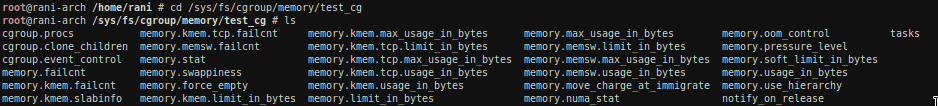
\includegraphics[width=1\textwidth]{img/cgroup_memory_ls.png}
			\caption{Archivos asociados al grupo \texttt{test\_cg} una vez lo creamos}
		\end{center}
	\end{figure}

	\pagebreak
	
	\noindent Si quisiéramos establecer un límite en el uso de memoria, tendríamos que escribir en el archivo \texttt{memory.limit\_in\_bytes}, a modo de ejemplo, establecemos un límite de 50MB. Esto se haría tal que:
	\begin{verbatim}
echo 50000000 > /sys/fs/cgroup/memory/<NombreGrupo>/memory.limit_in_bytes
	\end{verbatim}

	\noindent Para comprobar el funcionamiento de este límite de memoria, vamos a asociarle un programa escrito en Python que consume mucha memoria RAM de golpe. El programa en cuestión vendría dado por el siguiente código:
	\begin{lstlisting}[language=Python, caption={Programa en Python que consume 4 GB de RAM}]
#!/usr/bin/python
import numpy

print("cgroup testing program (memory limit)")
result = [numpy.random.bytes(1024*1024) for x in range(1024*4)]
print("RAM used: {}M".format(len(result)))
	\end{lstlisting}

	\noindent Ejecutamos el programa, y comprobamos como la salida por consola es tal que: 
	
	\begin{figure}[h!]
		\begin{center}
			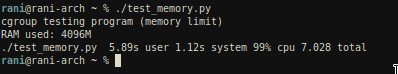
\includegraphics[width=0.7\textwidth]{img/cgroup_python1.png}
			\caption{Salida tras ejecutar el programa de Python sin limitar}
			\label{img: cgroup python 1}
		\end{center}
	\end{figure}

	\noindent Sin embargo, ahora vamos a proceder a limitar ese mismo programa en memoria. Para ello, vamos a añadir el PID asociado a la ejecución de dicho programa al siguiente archivo (ejecutando el script \texttt{./test\_memory.py \&}, nos aparece el PID):
	\begin{verbatim}
echo 62482 > /sys/fs/cgroup/memory/test_cg/cgroup.procs
	\end{verbatim}
	
	\noindent De esta manera ya estaríamos limitando la memoria de ese programa en concreto. Al limitarlo, podemos comprobar como la salida en consola es tal que: 
	
	\begin{figure}[h!]
		\begin{center}
			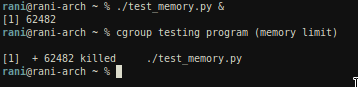
\includegraphics[width=0.7\textwidth]{img/cgroup_python2.png}
			\caption{Salida tras ejecutar el programa de Python, una vez limitado}
			\label{img: cgroup python 2}
		\end{center}
	\end{figure}

	\pagebreak
	
	\noindent Como podemos comprobar en las imágenes [\ref{img: cgroup python 1}] y [\ref{img: cgroup python 2}], la salida del programa no coincide. Esto es debido a que como el programa Python ha superado el límite establecido para su grupo, \texttt{cgroups} cerrado bruscamente dicho programa, por lo tanto no nos aparece la memoria consumida por el programa, solo se nos notifica que el proceso con PID 62482 ha pasado a estado ``\textit{killed}''.
	
	\addvspace{60px}
	
	\begin{figure}[h!]
		\begin{center}
			% https://8gwifi.org/docs/linux-namespace.jsp
			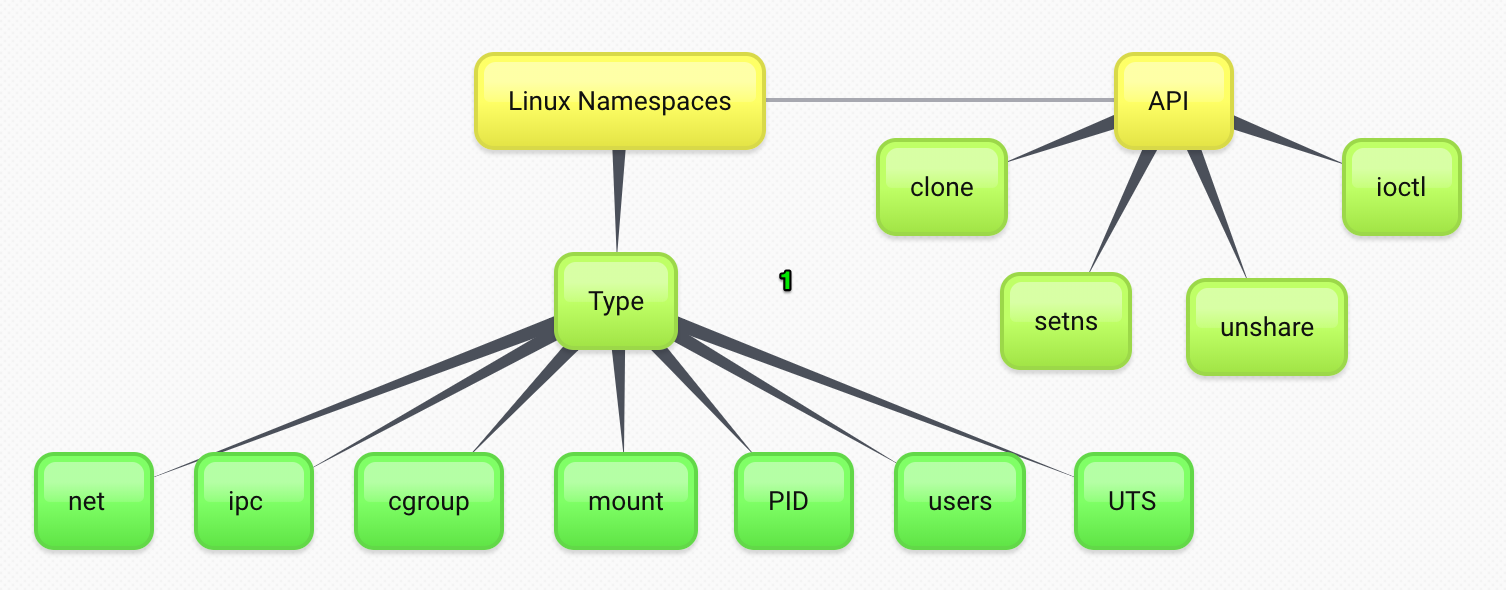
\includegraphics[width=1\textwidth]{img/linux-namespace1.png}
			\caption{Diferentes namespaces en Linux y su API de acceso. (\ref{bib:img1})}
		\end{center}
	\end{figure}
	
	
	\pagebreak
	\subsubsection{Time}
	\par \noindent Por último, nos queda el namespaces asociado al tiempo. Este namespace fue propuesto para que se incorporara al kernel de Linux en 2018 y en enero de 2020 fue añadido a la versión mainline de Linux. Apareció en la release 5.6 del kernel de Linux. \\
	
	\par \noindent El namespace time, permite que por cada namespace que tengamos, podamos crear desfases entre los relojes monotónicos (CLOCK\_MONOTONIC) y de boot (CLOCK\_BOOTTIME), de la máquina host. Esto permite que dentro de los contendores se nos permita cambiar la fecha y la hora, sin tener que modificar la hora del sistema host. Además, supone una capa más de seguridad, ya que no estamos vinculando directamente la hora a los relojes físicos de nuestro sistema. [\ref{bib:time ns kernel}]\\
	
	\par \noindent Un namespace de tipo time, es muy similar al namespace de tipo PID en la manera de como lo creamos. Utilizamos el comando unshare -T, y mediante una systemcall se nos creará un nuevo time namespace, pero no lo asocia directamente con el proceso. Tenemos que utilizar setns para asociar un proceso a un namespace, además todos los procesos dependientes también tendrán asignado dicho namespace. 
	
	\addvspace{80px}
	
	%\begin{figure}[h]
	%	\begin{center}
	%		% https://twitter.com/b0rk/status/1240364585766576128/photo/1
	%		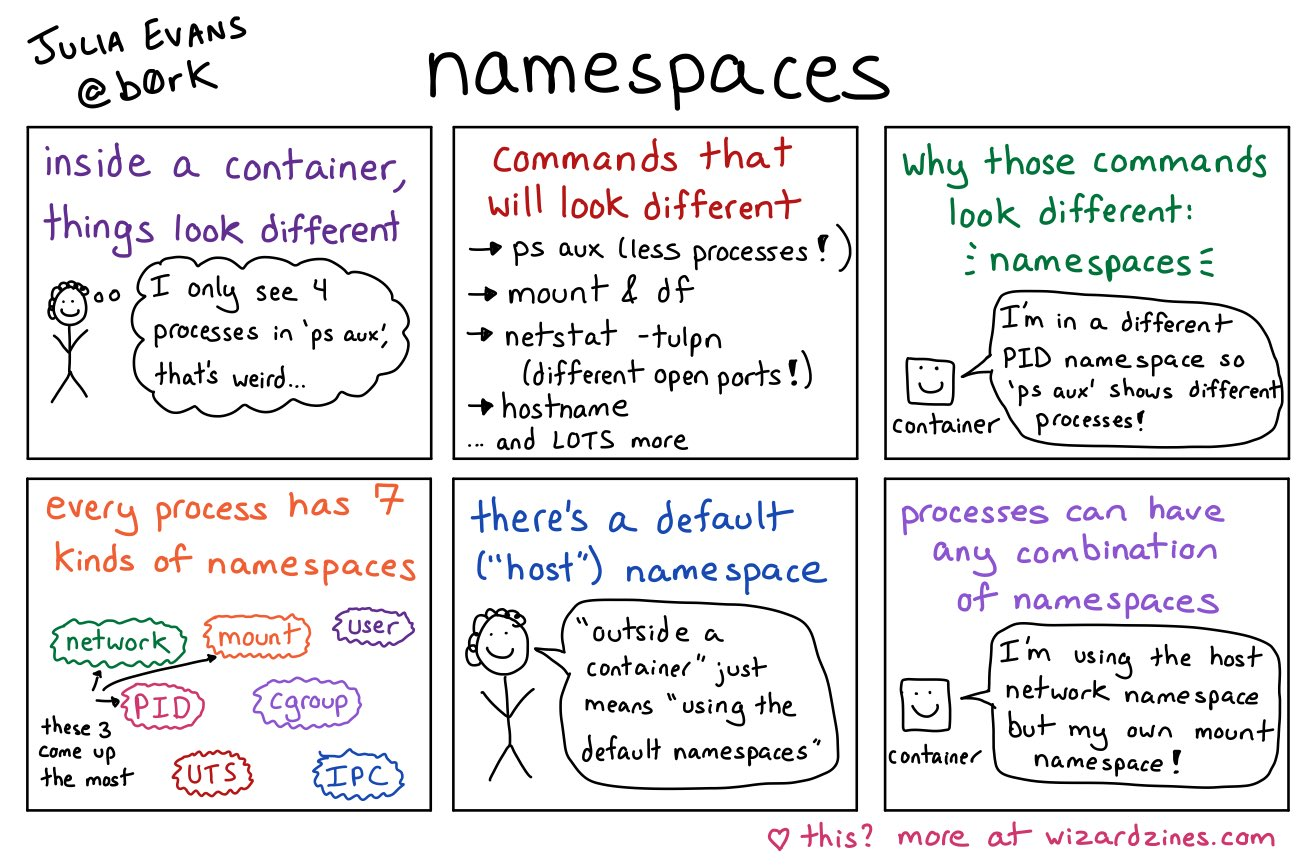
\includegraphics[width=0.8\textwidth]{img/how_containers_work.jpg}
	%		\caption{Como funcionan los contenedores. (\ref{bib:img2})}
	%	\end{center}
	%\end{figure}
	
	\pagebreak
	
	\subsection{Ejemplo de uso de 'netns' usando comando \texttt{ip}}
	\noindent En este apartado, vamos a detallar un ejemplo de como funciona el comando IP manejando los 'network namespaces'.\\
	
	\noindent Creamos los \textit{network namespaces}, en este caso, con nombre h1 y h2. El sistema no crea directamente el namespace, lo que en realidad hace es definirlos en el sistema. El \textit{network namespace} se crea cuando una aplicación se asocia a el.
	\begin{verbatim}
$ ip netns add h1
$ ip netns add h2
	\end{verbatim}

	\noindent Si utilizamos el comando \texttt{ip netns}, nos mostrará los netns existentes. Como es un sub-comando de \texttt{ip}, muestra los ns que el comando \texttt{lsns} no muestra. \\
	
	\noindent Procedemos a asociar una aplicación a cada netns. Utilizamos \texttt{bash}.
	\begin{verbatim}
$ ip netns exec h1 bash
$ ip netns exec h2 bash
	\end{verbatim}

	\noindent Ahora, si que podemos utilizar el comando \texttt{lsns}. Comprobamos que si nos aparecen los ns que hemos creado, cosa que antes de asociar una aplicación al ns, no pasaba. \\
	
	\noindent El comando \texttt{ip} crea automaticamente un \textit{nsfs} para poder colocar los archivos de configuración del \textit{netns}. Para ello, debe crearse el directorio \texttt{/etc/netns/h1} y poner en el los archivos de configuración de la red.
	\begin{verbatim}
$ mkdir /etc/netns/h1
$ echo "nameserver 8.8.8.8" > /etc/netns/h1/resolv.conf
	\end{verbatim}

	\noindent En este momento, tenemos el ns configurado con DNS. Nos quedaría realizar la conexión entre el ethernet físico de nuestro \textit{host} y las interfaces de nuestros namespaces. Para ello, vamos a utilizar un conmutador virtual, en este caso Open vSwitch.
	\begin{verbatim}
$ systemctl enable --now openvswitch.service
	\end{verbatim}

	\noindent Creamos un \textit{brige} utilizando el OpenvSwitch.
	\begin{verbatim}
$ $ ovs-vsctl add-br s1
	\end{verbatim}

	\noindent Utilizando el comando \texttt{ip}, creamos las interfaces virtuales de ethernet y las asignamos a sus namespaces.
	\begin{verbatim}
$ ip link add h1-eth0 type veth peer name s1-eth1
$ ip link add h2-eth0 type veth peer name s1-eth2
$ ip link set h1-eth0 netns h1
$ ip link set h2-eth0 netns h2
	\end{verbatim}

	\pagebreak
	
	\noindent Utilizando el comando \texttt{ovs-vsctl}, asignamos al \textit{bridge} el otro par ethernet que hemos creado para cada namespace.
	\begin{verbatim}
$ ovs-vsctl add-port s1 s1-eth1
$ ovs-vsctl add-port s1 s1-eth2
	\end{verbatim}

	\noindent Verificamos que el controlador sea \textit{standalone}, así el switch se comportará como un \textit{learning-switch}.
	\begin{verbatim}
$ ovs-vsctl set-fail-mode br0 standalone
	\end{verbatim}

	\noindent Como la conexión es desde localhost al exterior, entendemos que es una conexión fuera de banda.
	\begin{verbatim}
$ ovs-vsctl set controller br0 connection-mode=out-of-band
	\end{verbatim}

	\noindent En este momento, tenemos todos configurado a falta de habilitar las diferentes interfaces de nuestra topología.
	\begin{verbatim}
$ ip netns exec h1 ip link set h1-eth0 up
$ ip netns exec h1 ip link set lo up
$ ip netns exec h1 ip add add 10.0.0.1/24 dev h1-eth0
$ ip netns exec h2 ip link set h2-eth0 up
$ ip netns exec h2 ip link set lo up
$ ip netns exec h2 ip add add 10.0.0.2/24 dev h2-eth0
$ ip link set s1-eth1 up
$ ip link set s1-eth2 up
	\end{verbatim}

	\noindent Ahora tenemos todas las interfaces configuradas, el switch activado y el sistema interconectado, por lo que podemos ejecutar un ping en una de las terminales de los namespaces para verificar la topología.
	\begin{verbatim}
$ ip netns exec h1 ping -c4 10.0.0.2
	\end{verbatim}

	\noindent Si queremos revertir todas las configuraciones que hemos hecho, lo que tenemos que hacer es ejecutar los siguientes comandos:
	\begin{verbatim}
$ ovs-vsctl del-br s1
$ ip link delete s1-eth1
$ ip link delete s1-eth2
$ ip netns del h1
$ ip netns del h2
	\end{verbatim}

	\pagebreak

	\subsection{Ejemplo de uso de 'netns' usando comando \texttt{unshare}}
	\noindent En el ejemplo anterior, utilizabamos el comando \texttt{ip} para manejar los netns, sin embargo, eso nos limitaba los tipos namespaces que queriamos asignar a nuestro namespace. En contra partida a esto, el comando \texttt{unshare} nos da más libertad a la hora de crear los namespaces. \\
	
	\noindent Utilizando \texttt{unshare}, no podemos ponerle un nombre, pero sí que nos permite asociarlo a un archivo, que montará con tipo bind. Esto nos permitirá utilizar en namespace aunque no haya ningún proceso corriendo en el, para ello podemos utilizar el comando \texttt{nsenter}.
	\begin{verbatim}
$ touch /var/net-h1
$ touch /var/uts-h1
$ unshare --net=/var/net-h1 --uts=/var/uts-h1 /bin/bash
	\end{verbatim}

	\noindent Utilizando el comando \texttt{nsenter} podemos ejecutar comandos dentro del namespace.
	\begin{verbatim}
$ nsenter --net=/var/net-h1 --uts=/var/uts-h1 hostname h1
$ nsenter --net=/var/net-h1 --uts=/var/uts-h1 ip address
	\end{verbatim}

	\noindent Para destruir el namespace, lo que tendremos que hacer es desmontar los archivos asignados a dicho namespace.
	\begin{verbatim}
$ umount /var/net-h1
$ umount /var/uts-h1
	\end{verbatim}

	\noindent Como será común necesitar más de un namespace, de ahora en adelante tendremos que utilizar los comandos \texttt{unshare} y \texttt{nsenter}.

	\pagebreak
	
	\section{Virtualización ligera y contenedores}
	\noindent En este capítulo vamos a trabajar el concepto de virtualización ligera, que ya introdujimos en el apartado \ref{sect: virt ligera}, pero esta vez aplicando los conceptos de \texttt{namespaces} del apartado anterior. Además, presentaremos el concepto de \textit{contenedor}, y como supone una de las piezas más importantes para la virtualización tal y como hoy día la conocemos. \\
	
	\noindent Recuperando la definición de \textbf{virtualización ligera}, entendemos este tipo de virtualización como aquella que \textbf{se realiza a nivel de sistema operativo}, permitiendo la coexistencia de diferentes espacios aislados entre sí. En dichos espacios, podremos ejecutar de manera aislada nuestras aplicaciones. Como punto en común, todos los espacios aislados que creemos, \textbf{utilizarán} como base \textbf{el mismo \texttt{kernel}}. La tecnología clave para realizar esta virtualización serán los diferentes \texttt{namespaces}, comentados en el apartado \ref{sect: espacio nombres}, que podremos combinar a nuestro gusto con el fin de crear un espacio aislado con todos los recursos necesarios para satisfacer las necesidades de nuestra aplicación. \\
	
	\noindent La principal ventaja que encontramos al utilizar \texttt{namespaces}, respecto a otro tipo de virtualizaciones como podrían ser las máquinas virtuales, es el aprovechamiento de los recursos de la máquina host. Al tener todos el mismo kernel, evitamos tener por duplicados los kernels para cada una de las instancias a realizar, ahorrando ciclos de CPU, como espacio en RAM.\\
	
	\noindent Por otro lado, tenemos el concepto de \textbf{contenedor}. Entendemos contenedor, en el ambito de la virtualización, como una abstracción a alto nivel de un sistema aislado creado utilizando \texttt{namespaces} y \texttt{cgroups}. Por lo tanto, si el kernel nos da la posibilidad de trabajar a bajo nivel utilizando dichos \texttt{namespaces}, en este caso, buscamos ir más allá y encapsular dicho espacio aislado en unas APIs de alto nivel, que sean mucho más fáciles de entender y de implementar. Tenemos muchos ejemplos de sistemas que trabajan con contenedores, y muchos de ellos implementados en una amplia variedad de lenguajes [\ref{bib:container is a lie}]. Algunos de los más importantes son:
	\begin{itemize}
		\item \texttt{LXC}, LinuX Containers, escrito en C: \url{https://linuxcontainers.org/}
		\item \texttt{Docker}, escrito en Go: \url{https://www.docker.com/}
		\item \texttt{Podman}, escrito en Go: \url{https://podman.io/}
		\item \texttt{systemd-nspawn}, escrito en C, implementado dentro de \texttt{systemd}: \url{https://github.com/systemd/systemd}
		\item \texttt{Vagga}, escrito en Rust: \url{https://github.com/tailhook/vagga}
	\end{itemize}

	\noindent Por último, es interesante comentar el concepto de \texttt{chroot}, ya que muchas de estas abstracciones de los \texttt{namespaces} hacen uso de esta técnica para su funcionamiento. Un \texttt{chroot} es una operación Unix que permite cambiar la ruta aparente de un directorio para un usuario en específico. Un proceso ejecutado después de realizar un \texttt{chroot} solo tendrá acceso al nuevo directorio definido y a sus subdirectorios, esta operación recibe el nombre de \texttt{chroot jail}, ya que los procesos no pueden leer ni escribir fuera del nuevo directorio. Este método suele ser de gran utilidad en virtualizaciones a nivel de kernel, es decir, virtualización ligera o contenedores. [\ref{bib: chroot jail}]
	
	\pagebreak
	
	\subsection{Creando nuestro propio ``contenedor''}
	
	\pagebreak
	
	\subsection{Contenedores \texttt{LXC}}
	\noindent En ese apartado vamos a comentar la aplicación de contenedores LXC, LinuX Containers. Como bien hemos comentado en el apartado anterior, LXC consiste en una virtualización a nivel de sistema operativo (virtualización ligera), creada por el proyecto \url{linuxcontainers.org}, con el objetivo de poder ejecutar diferentes espacios aislados (contenedores) utilizando un único host, lo llamaremos LXC host. Aunque pueda parecer que estamos ante una técnica de virtualización basada en máquinas virtuales, se trata de espacios virtuales, en los que cada uno dispone de su propia CPU, memoria, redes, etc. Esto lo consigue gracias al uso de los \texttt{namespaces} y los \texttt{cgroups} en el host LXC. [\ref{bib: LXC arch}]. Algunas de las características más destacables son:
	\begin{itemize}
		\item Utiliza mount namespace para conseguir la estructura de directorios propia de una distribución de Linux.
		\item El proceso asignado a cada namespaces es el \texttt{init}, por lo tanto tendremos un proceso de arranque del sistema.
		\item Tiene sus propios usuarios, incluido un usuario root.
		\item Una vez dentro del contenedor, podemos instalar aplicaciones utilizando el gestor de paquetes de la distribución (\texttt{apt}, \texttt{zipper}, \texttt{pacman}, etc...)
	\end{itemize}

	\begin{figure}[h]
		\begin{center}
			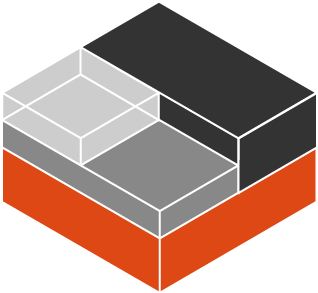
\includegraphics[width=0.2\textwidth]{img/lxc_logo.png}
			\caption{Logotipo del proyecto \url{linuxcontainers.org} [\ref{bib_img: lxc logo}]}
		\end{center}
	\end{figure}

	\noindent \textbf{\large Contenedores sin privilegios}\\

	\noindent Una característica muy importante de este tipo de contenedores es que permiten la posibilidad de configurar contenedores de dos tipos: contenedores con privilegios y contenedores sin privilegios. Esto es importante ya que si definimos un contenedor con privilegios, hay ciertas acciones que nos permitirían realizar comandos en el host. En el caso de que nuestro contenedor sea distribuido por terceros, puede suponer un problema grave de seguridad, ya que un atacante podría tomar el control de nuestro contenedor, y por consiguiente, también podría acceder a la información del host. Es por esto por lo que surge el concepto de contenedores sin privilegios (\textit{unprivileged containers}), considerados como una técnica mucho más segura ya que disponen de un nivel añadido de aislamiento respecto al host. La clave reside en ``mapear'' el UID del usuario \texttt{root} de nuestro contenedor a un UID del host que no tenga permisos de administrador. Por lo tanto, si un atacante consigue acceder a nuestro contenedor, y pudiera acceder al host, se vería con que no tiene permisos para realizar ninguna acción. [\ref{bib: LXC arch}]
	
	\pagebreak
	
	\noindent \textbf{\large Tipos de configuración de red en el host}\\
	
	\noindent LXC soporta dos tipos de conexiones virtuales de red. Estas son las siguientes: 
	\begin{itemize}
		\item NAT bridge. En este modo, LXC tiene su propio bridge (\texttt{lxcbr0}) que funciona en conjunto con las aplicaciones \texttt{dnsmasq} e \texttt{iptables} del host, dando lugar a que se puedan utilizar servicios red como DNS, DHCP y NAT dentro del propio contenedor.
		\item Host bridge. En este modo, ese necesario que el host configure su propio bridge para dar servicio a las aplicaciones que creamos pertinentes. Esta opción nos permite mucha flexibilidad a la hora de interconectar nuestros contenedores para una funcionalidad específica.
	\end{itemize}


	\vspace{20px}

	\noindent \textbf{\large Utilizar NAT bridge en un contenedor}\\

	\noindent A modo de ejemplo, si quisiéramos utilizar redes tipo NAT bridge en un contenedor [\ref{bib: LXC arch}], primero tendríamos que crear el archivo \texttt{/etc/default/lxc-net} con el siguiente contenido:
	\begin{lstlisting}[language=Bash, caption={Configuración interfaz NAT bridge en LXC}]
# Leave USE_LXC_BRIDGE as "true" if you want to use lxcbr0 for your
# containers.  Set to "false" if you'll use virbr0 or another existing
# bridge, or mavlan to your host's NIC.
USE_LXC_BRIDGE="true"

# If you change the LXC_BRIDGE to something other than lxcbr0, then
# you will also need to update your /etc/lxc/default.conf as well as the
# configuration (/var/lib/lxc/<container>/config) for any containers
# already created using the default config to reflect the new bridge
# name.
# If you have the dnsmasq daemon installed, you'll also have to update
# /etc/dnsmasq.d/lxc and restart the system wide dnsmasq daemon.
LXC_BRIDGE="lxcbr0"
LXC_ADDR="10.0.3.1"
LXC_NETMASK="255.255.255.0"
LXC_NETWORK="10.0.3.0/24"
LXC_DHCP_RANGE="10.0.3.2,10.0.3.254"
LXC_DHCP_MAX="253"
# Uncomment the next line if you'd like to use a conf-file for the lxcbr0
# dnsmasq.  For instance, you can use 'dhcp-host=mail1,10.0.3.100' to have
# container 'mail1' always get ip address 10.0.3.100.
#LXC_DHCP_CONFILE=/etc/lxc/dnsmasq.conf

# Uncomment the next line if you want lxcbr0's dnsmasq to resolve the .lxc
# domain.  You can then add "server=/lxc/10.0.3.1' (or your actual $LXC_ADDR)
# to your system dnsmasq configuration file (normally /etc/dnsmasq.conf,
# or /etc/NetworkManager/dnsmasq.d/lxc.conf on systems that use NetworkManager).
# Once these changes are made, restart the lxc-net and network-manager services.
# 'container1.lxc' will then resolve on your host.
#LXC_DOMAIN="lxc"
	\end{lstlisting}

	\pagebreak

	\noindent Ahora, necesitamos modificar la \textit{template} del contenedor LXC para que utilice la interfaz que hemos configurado. Modificamos la plantilla con ruta \texttt{/etc/lxc/default.conf} tal que:
	\begin{lstlisting}[language=Bash, caption={Configuración contenedor LXC para usar NAT bridge}]
lxc.net.0.type = veth
lxc.net.0.link = lxcbr0
lxc.net.0.flags = up
lxc.net.0.hwaddr = 00:16:3e:xx:xx:xx
	\end{lstlisting}

	\noindent Para que todos estos cambios se realicen, es necesario que tengamos activado el servicio \texttt{lxc-net.service}.
	\begin{verbatim}
> sudo systemctl enable lxc-net.service
> sudo systemctl start lxc-net.service
	\end{verbatim}

	\vspace{20px}

	\noindent \textbf{\large Crear un contenedor con privilegios utilizando LXC}\\
	
	\noindent Si decidimos crear un contenedor con privilegios, tendríamos que seguir los siguientes pasos [\ref{bib: crear LXC}]:
	\begin{lstlisting}[language=Bash, caption={Crear un contenedor con privilegios en LXC}]
sudo lxc-create --template download --name <NombreContenedor>
	\end{lstlisting}

	\noindent Con este comando, LXC nos preguntará de manera interactiva por un \texttt{root filesystem} para el contenedor a descargar, además de la distribución elegida, la versión o la arquitectura. Si queremos hacerlo de manera que no sea interactivo, podemos crear el contenedor tal que:
	\begin{lstlisting}[language=Bash, caption={Crear un contendor con privilegios en LXC, modo no interactivo}]
sudo lxc-create --template download --name <NombreContenedor> -- --dist debian --release stretch --arch amd64
	\end{lstlisting}

	\noindent De esta manera, ya tendríamos creado nuestro contenedor. Para poder manejar dichos contenedores, es conveniente conocer los comandos disponibles por LXC. Algunos de los más importantes son los siguientes [\ref{bib: crear LXC}]:
	\begin{itemize}
		\item \texttt{sudo lxc-ls --fancy}. Lista los contenedores disponibles por el host.
		\item \texttt{sudo lxc-info --name <NombreContenedor>}. Permite conocer la información de un contenedor específico.
		\item \texttt{sudo lxc-attach --name <NombreContenedor>}. Nos conecta directamente con la shell de nuestro contenedor.
		\item \texttt{sudo lxc-start --name <NombreContenedor> --daemon}. Permite arrancar el contenedor.
		\item \texttt{sudo lxc-stop --name <NombreContendor>}. Permite parar un contenedor que esté en ejecución.
		\item \texttt{sudo lxc-destroy --name <NombreContenedor>}. Elimina un contenedor, incluido su directorio \texttt{root}.
	\end{itemize}
	
	\pagebreak
	
	\noindent Una vez creamos el contenedor, es interesante modificar su configuración para asignarle una interfaz de red. Esto lo haremos modificando el archivo config con ruta: 
	\begin{verbatim}
/var/lib/lxc/<NombreContenedor>/config
	\end{verbatim}
	\noindent Añadiremos la siguiente configuración para que utilice el \texttt{NAT bridge} que definimos con anterioridad, además de permitir la ejecución de aplicaciones tipo X11, utilizando xorg (aplicaciones con interfaz gráfica) [\ref{bib: xorg arch wiki}].
	\begin{lstlisting}[language=Bash, caption={Configuración interfaz NAT bridge y aplicaciones X a un contenedor LXC}]
# Network configuration (bridge)
lxc.net.0.type = veth
lxc.net.0.veth.pair = veth_containerLXC
lxc.net.0.flags = up
lxc.net.0.ipv4.address = 172.16.27.2/24

## for xorg
lxc.mount.entry = /dev/dri dev/dri none bind,optional,create=dir
lxc.mount.entry = /dev/snd dev/snd none bind,optional,create=dir
lxc.mount.entry = /tmp/.X11-unix tmp/.X11-unix none bind,optional,create=dir,ro
lxc.mount.entry = /dev/video0 dev/video0 none bind,optional,create=file
	\end{lstlisting}
	
	\noindent Ahora ya tenemos listo el contenedor para arrancarlo, solo nos quedaría asignar una IP válida al host, que también está dentro del \texttt{bridge} de LXC. Para ello, ejecutaremos:
	\begin{lstlisting}[language=Bash, caption={Asignar IP al host LXC y arrancar un contenedor}]
ip link add 172.16.27.1/24 dev veth_containerLXC
sudo lxc-start --name <NombreContenedor>
sudo lxc-attach --name <NombreContenedor>

# Para ejecutar interfaz grafica
startx
	\end{lstlisting}

	\vspace{20px}

	\noindent \textbf{\large Crear un contenedor sin privilegios utilizando LXC}\\
	
	\noindent En el caso de optar por la opción más segura, que es la de crear un contenedor sin privilegios en el host. Tendremos que realizar una serie de configuraciones previas [\ref{bib: unprivileged LXC}]. La primera consistirá en crear un usuario sin privilegios para LXC:
	\begin{verbatim}
sudo useradd -s /bin/bash -c 'unprivileged lxc user' -m lxc_user
sudo passwd lxc_user
	\end{verbatim}

	\noindent Ahora, necesitamos buscar los valores de grupo (subgid) e identificación (subuid) del usuario creado, para ello ejecutamos lo siguiente:
	\begin{verbatim}
sudo grep lxc_user /etc/sub{gid,uid}
	\end{verbatim}

	\noindent Obteniendo por consola una salida similar a la siguiente:
	\begin{verbatim}
/etc/subgid:lxc_user:100000:65536
/etc/subuid:lxc_user:100000:65536
	\end{verbatim}

	\pagebreak
	
	\noindent Utilizando las mismas configuraciones de red que en el aparatado de contenedor con privilegios, procedemos a acceder al usuario asignado a LXC. Ejecutaremos el comando \texttt{id} para conocer los diferentes \texttt{uid} y \texttt{gid} asignados.
	\begin{verbatim}
su lxc_user
id
	\end{verbatim}

	\noindent Tendremos una salida similar a:
	\begin{verbatim}
uid=1002(lxc_user) gid=1002(lxc_user) groups=1002(lxc_user)
	\end{verbatim}

	\noindent El siguiente paso sería crear los directorios de configuración de LXC, y copiar la configuración \textit{default} a dichos directorios.
	\begin{verbatim}
mkdir -p /home/lxc_user/.config/lxc
cp /etc/lxc/default.conf /home/lxc_user/.config/lxc/default.conf
	\end{verbatim}

	\noindent Por último, tendríamos que modificar dicho archivo para realizar un ``mapeo de permisos''. Con el fin de asignar la ejecución del contenedor al usuario LXC que acabamos de crear. Al final del archivo \texttt{default.conf} que acabamos de copiar, añadimos lo siguiente:
	\begin{lstlisting}[language=Bash, caption={Configuración para mapear UID y GID para un contenedor sin privilegios en LXC}]
lxc.id_map = u 0 100000 65536
lxc.id_map = g 0 100000 65536
	\end{lstlisting}

	\noindent Una vez realizados todos estos pasos, ya podríamos crear nuestro contenedor sin privilegios. Lo haríamos de manera similar que en el apartado anterior, es decir utilizando el comando \texttt{lxc-create}. Además, también será importante modificar el archivo \texttt{config} de nuestro contenedor para asignar la interfaz de red y permitir la ejecución de aplicaciones con interfaz gráfica.
	
	\pagebreak
	
	\subsection{Contenedores \texttt{Docker}}
	
	\pagebreak

	\section{Caso práctico: Virtualización para simulación de redes}
	\subsection{Interconexión física de diferentes red virtuales}
	\subsection{Evaluación de prestaciones}
	
	\pagebreak
	
	\section{Conclusiones}
	
	\subsection{Propuestas futuras}
	
	% Propuestas futuras
	% Openflow OKO

	%%% Bibliography
	\pagebreak
	\section*{Bibliografía}
	\addcontentsline{toc}{section}{Bibliografía}
	\subsection*{Enlaces y referencias}
	\addcontentsline{toc}{subsection}{Enlaces y referencias}
	%%\hyperref[bib:link1]{\emph{Reference of bibliography}}
	\begin{enumerate}
		%1
		\item 
		\label{bib:ns overview} \href{https://lwn.net/Articles/531114/}{\textit{Namespaces}}
		
		%2
		\item 
		\label{bib:ns tutorial1} \href{https://laurel.datsi.fi.upm.es/~ssoo/SOA/namespaces.html}{Tutorial: Espacio de nombres en Linux}
		
		%3
		\item 
		\label{bib:time ns} \href{https://www.phoronix.com/scan.php?page=news_item&px=Linux-Time-Namespace-Coming}{\textit{Time namespaces coming to linux}}
		
		%4
		\item 
		\label{bib:container is a lie} \href{https://platform.sh/blog/2020/the-container-is-a-lie/}{\textit{Container is a lie. Namespaces}}
		
		%5
		\item 
		\label{bib:link5} \href{https://locurastecnicas.blogspot.com/2020/09/linux-namespaces-y-cgroups.html}{\textit{Namespaces.} Uso de \textit{cgroups}.}
		
		%6
		\item 
		\label{bib:link6} \href{https://www.youtube.com/watch?v=_WgUwUf1d34}{\textit{Introduction to Network Namespaces}}
		
		
		%7
		\item
		\label{bib:link7} \href{https://www.redhat.com/sysadmin/mount-namespaces}{\textit{Build a container by hand: the mount namespace}}
		
		
		%8
		\item
		\label{bib:pid wikipedia}
		\href{https://en.wikipedia.org/wiki/Process_identifier}{Indentificador de procesos (\textit{process id})}
		
		
		%9
		\item
		\label{bib:link9}
		\href{https://www.redhat.com/sysadmin/linux-pid-namespaces}{\textit{Linux PID namespaces work with containers}}
		
		%10
		\item
		\label{bib:link10}
		\href{https://blogs.igalia.com/dpino/2016/04/10/network-namespaces/}{\textit{Network Namespaces}}
		
		%11
		\item
		\label{bib:virtual interface list}
		\href{https://developers.redhat.com/blog/2018/10/22/introduction-to-linux-interfaces-for-virtual-networking#veth}{\textit{Introduction to Linux interfaces for virtual networking}}
		
		
		%12
		\item
		\label{bib:link12}
		\href{https://elpuig.xeill.net/Members/vcarceler/articulos/introduccion-a-los-grupos-de-control-cgroups-de-linux}{\textit{Introducción a los grupos de control (cgroups) de Linux}}
		
		%13
		\item
		\label{bib:time ns kernel}
		\href{https://git.kernel.org/pub/scm/linux/kernel/git/tip/tip.git/commit/?h=timers/core&id=769071ac9f20b6a447410c7eaa55d1a5233ef40c}{\textit{Time namespaces}}
		
		%14
		\item
		\label{bib:example netns veth}
		\href{https://blog.scottlowe.org/2013/09/04/introducing-linux-network-namespaces/}{\textit{Network namespaces. Assign and configure}}
		
		
		%15
		\item
		\label{bib:configure host-only}
		\href{https://www.tecmint.com/network-between-guest-vm-and-host-virtualbox/}{How to configure Network Between Guest VM and Host in Virtualbox}
		
		
		%16
		\item
		\label{bib:install ansible}
		\href{https://www.cyberciti.biz/faq/how-to-install-ansible-on-fedora-for-it-and-server-automation/}{How to install ansible on fedora for it and server automation}
		
		%17
		\item
		\label{bib: herramientas virtualizacion}
		\href{https://www.uv.es/sto/charlas/2010_CIM/hvl-cim-2010.html/index.html}{\textit{Herramientas de virtualización libres para sistemas GNU/Linux}}
		
		%18
		\item
		\label{bib: what is nfv}
		\href{https://www.ciena.com/insights/articles/What-is-NFV-prx.html}{W\textit{hat is Network Function Virtualization(NFV)?}}
		
		%19
		\item
		\label{paper nfv 2012}
		\href{https://portal.etsi.org/nfv/nfv_white_paper.pdf}{NFV white paper}
		
		%20
		\item
		\label{youtube: nfv y sdn cristina}
		\href{https://www.youtube.com/watch?v=3JEAK66wujg}{Youtube: NFV y SDN: las redes del futuro y del presente - Cristina Santana | T3chFest 2018}
		
		%21
		\item
		\label{servers running linux}
		\href{https://hostingtribunal.com/blog/linux-statistics/}{Percentage of server that run in Linux}
		
		%22
		\item
		\label{bib: vmware sdn}
		\href{https://www.vmware.com/es/topics/glossary/content/software-defined-networking.html}{¿Qué son las redes definidas por software (SDN)?}
		
		%23
		\item
		\label{bib: vmware nfv}
		\href{https://www.vmware.com/es/topics/glossary/content/virtual-networking.html}{¿Qué son las redes virtuales?}
		
		%24
		\item
		\label{bib: udev archwiki}
		\href{https://wiki.archlinux.org/title/Udev}{\textit{Arch Linux Wiki: udev}}
		
		%25
		\item
		\label{bib: systemd networkd v197}
		\href{https://www.freedesktop.org/wiki/Software/systemd/PredictableNetworkInterfaceNames/}{Predictable Network Interface Names}
		
		%26
		\item
		\label{bib: open vswitch}
		\href{https://www.openvswitch.org/}{Open vSwitch}
		
		%27
		\item
		\label{bib: veth netns ovs}
		\href{https://matthewarcus.wordpress.com/2018/02/04/veth-devices-network-namespaces-and-open-vswitch/}{Veth Devices, Network Namespaces and Open vSwitch}
		
		%28
		\item
		\label{bib: 802.1ad}
		\href{http://www.microhowto.info/tags/802.1ad.html}{IEEE 802.1ad}
		
		%29
		\item
		\label{bib: FS QinQ}
		\href{https://img-en.fs.com/file/user_manual/s3800-series-qinq-operation.pdf}{FS.COM QinQ Operation}
		
		%30
		\item
		\label{bib: openwrt virtual network interfaces}
		\href{https://openwrt.org/docs/guide-developer/networking/network.interfaces}{OpenWrt: Linux Network Interfaces}
		
		%31
		\item
		\label{bib: sdn y nfv}
		\href{https://comparacloud.com/servicios-clouds/sdn-y-nfv/}{SDN \& NFV}
		
		%32
		\item
		\label{bib: tun vs tap}
		\href{https://www.gabriel.urdhr.fr/2021/05/08/tuntap/}{TUN/TAP interface (on Linux)}
		
		%33
		\item
		\label{bib: tunctl + ip}
		\href{https://developpaper.com/creating-tap-tun-devices-with-ip-tuntap-and-tunctl-as-detailed-in-linux-network-tools/}{Creating tap/tun devices with IP tuntap and tunctl as detailed in Linux network tools}
		
		%34
		\item
		\label{bib: code tuntap.c}
		\href{https://programmerclick.com/article/45831226469/}{Principio de diseño del controlador TUN/TAP de la tarjeta virtual}
		
		%35
		\item
		\label{bib: cgroups}
		\href{https://www.nginx.com/blog/what-are-namespaces-cgroups-how-do-they-work/}{What are namespaces cgroups how do they work}
		
		%36
		\item
		\label{bib: virt ligera}
		\href{https://upcommons.upc.edu/handle/2117/78028?show=full}{TFG. Evaluación de prestaciones mediante NVF}
		
		%37
		\item
		\label{bib: sock}
		\href{http://www.icir.org/christian/sock.html}{Aplicación sock}
		
		%38
		\item
		\label{bib: chroot jail}
		\href{https://phoenixnap.com/kb/chroot-jail}{What is chroot jail and How to Use it?}
		
		%39
		\item
		\label{bib: LXC arch}
		\href{https://wiki.archlinux.org/title/Linux_Containers}{ArchLinux Wiki: Linux Containers}
		
		%40
		\item
		\label{bib: crear LXC}
		\href{https://ubuntu.com/server/docs/containers-lxc}{Ubuntu LXC}
		
		%41
		\item
		\label{bib: xorg arch wiki}
		\href{https://wiki.archlinux.org/title/xorg}{ArchLinux Wiki: Xorg}
		
		%42
		\item
		\label{bib: unprivileged LXC}
		\href{https://www.cyberciti.biz/faq/how-to-create-unprivileged-linux-containers-on-ubuntu-linux/}{How to create unprivileged LXC container}
		
		% X
		\item
		\label{bib: docker works namespaces}
		\href{https://www.youtube.com/watch?v=-YnMr1lj4Z8}{Youtube LiveOverflow: How Docker Works - Intro to Namespaces}
		
		% X
		%\item
		%\label{bib:link20}
		%\href{https://jsitech1.gitbooks.io/meet-docker/content/fundamentos_de_docker.html}{Fundamentos de Docker}
		
	\end{enumerate}

	\pagebreak

	\subsection*{Imágenes}
	\addcontentsline{toc}{subsection}{Imagenes}
	\begin{enumerate}
		%1
		\item
		\label{img: nfv vs classic}
		\href{https://portal.etsi.org/nfv/nfv_white_paper.pdf}{NFV white paper}
		
		%2
		\item
		\label{img: nfv vs classic 2}
		\href{https://www.ciena.com/insights/articles/What-is-NFV-prx.html}{W\textit{hat is Network Function Virtualization(NFV)?}}
		
		%3
		\item
		\label{img: sdn vs nfv osi}
		\href{https://comparacloud.com/servicios-clouds/sdn-y-nfv/}{SDN \& NFV}
		
		%4
		\item
		\label{img: frame ethernet 802.1ad}
		\href{https://img-en.fs.com/file/user_manual/s3800-series-qinq-operation.pdf}{FS.COM QinQ Operation}
		
		%4
		\item 
		\label{bib:img1}\href{https://8gwifi.org/docs/linux-namespace.jsp}{Namespaces y API de acceso.}
		
		%5
		\item
		\label{bib_img: tun tap}
		\href{https://en.wikipedia.org/wiki/TUN/TAP}{Wikipedia: TUN/TAP}
		
		%6
		\item
		\label{bib_img: comparativa virt}
		\href{https://www.slideshare.net/janghoonsim/docker-container-and-lightweight-virtualization}{Docker - container and lightweight virtualization}
		
		%7
		\item
		\label{bib_img: lxc logo}
		\href{https://linuxcontainers.org/}{Linux Containers Logotipo}
		
		%\item 
		%\label{bib:img2}\href{https://twitter.com/b0rk/status/1240364585766576128}{How containers work.}
		
		
	\end{enumerate}

	\pagebreak
	
	\pagebreak
	\section*{Anexos}
	\addcontentsline{toc}{section}{Anexos}
	\subsection*{Anexo 1. Instalación de \texttt{ansible} para automatizar una VM}
	\addcontentsline{toc}{subsection}{Anexo 1. Instalación \texttt{ansible}}
	\noindent En el caso de que queramos utilizar la herramienta ansible para configurar una VM, tendremos que seguir los siguientes pasos.
	\begin{enumerate}
		\item Asegurarnos de que tenemos instalado el programa en el host. La principal dependencia de \texttt{ansible} es \texttt{Python}. \\
		Para instalar \texttt{ansible} en diferentes distribuciones sería tal que:
		\begin{itemize}
			\item Ubuntu 21.04:
			\begin{lstlisting}[language=Bash, caption={Instalación \texttt{ansible} en Ubuntu}]
sudo apt install -y software-properties-common
sudo add-apt-repository --yes --update ppa:ansible/ansible
sudo apt update
sudo apt install -y ansible
			\end{lstlisting}
			
			\item Fedora 32:
			\begin{lstlisting}[language=Bash, caption={Instalación \texttt{ansible} en Fedora}]
sudo dnf update
sudo dnf install ansible
			\end{lstlisting}
			
			\item OpenSUSE:
			\begin{lstlisting}[language=Bash, caption={Instalación \texttt{ansible} en OpenSUSE}]
zypper in ansible
			\end{lstlisting}
			
			\item Arch Linux:
			\begin{lstlisting}[language=Bash, caption={Instalación \texttt{ansible} en Arch Linux}]
sudo pacman -S ansible
			\end{lstlisting} 
		\end{itemize}
		
		\item Creamos una clave SSH para utilizarla como método de autentificación con la maquina virtual. 
		\begin{lstlisting}[language=Bash, caption={Crear clave SSH para autenticación en VM}]
(host)$ ssh-keygen -t ed25519 -C "Host Ansible ssh key"
		\end{lstlisting}
		
		\pagebreak
		
		\item Utilizando nuestro gestor de máquinas virtuales, encendemos la VM. Es importante que nos aseguremos que tiene internet, por lo que configuramos que la interfaz de red sea de tipo \textit{NAT}. Dentro de la máquina, buscaremos que ip tiene asignada con el comando \texttt{ip address}. Desde este momento, dejaremos la máquina virtual encendida.
		
		\item Procedemos a copiar la clave pública SSH que hemos generado en el paso dos. Utilizamos el siguiente comando, sustituyendo con el usuario e IP específico de la máquina. Tendremos que configurar una red tipo \textit{Host-only network} para poder comunicarnos correctamente con nuestra máquina virtual, para ello podemos seguir los pasos detallados en [\ref{bib:configure host-only}]
		\begin{lstlisting}[language=Bash, caption={Copiar clave pública de \texttt{ansible} a VM}]
(host)$ ssh-copy-id -i $HOME/.ssh/id_ed25519.pub <user>@<IP VM>
		\end{lstlisting}

		\item En este momento ya podríamos conectar con la máquina virtual utilizando \texttt{ansible}. Sin embargo, por comodidad, lo que vamos a hacer es crear un archivo que funcione con inventario de servidores. Nos servirá para guardar las direcciones IP de los servidores en los que queremos ejecutar comandos remotos con \texttt{ansible}. Para ello, creamos un archivo \texttt{inventory}. Como ejemplo, dicho archivo puede ser tal que:
		\begin{lstlisting}[language=Bash, caption={Contenido del archivo \texttt{inventory} de \texttt{ansible}}]
## VMs locals 
[virtualbox]
10.0.100.1
10.0.100.2
			
## Server SSH
[server]
192.168.1.200
		\end{lstlisting}
		
		\item Para probar la conectividad. Nos aseguramos de que tenemos la máquina virtual encendida y que además, hemos copiado la clave ssh y tenemos su IP añadida a nuestro inventario. Después, procedemos a ejecutar el siguiente comando en la máquina host:
		\begin{verbatim}
			(host)$ ansible -i inventory -m ping
		\end{verbatim}
		\noindent En la consola nos aparecerá la información de cada uno de las IP que habrá probado para ejecutar el comando remoto \texttt{ping}.
	\end{enumerate}
	
	\pagebreak
	
	\subsection*{Anexo 2. Configuración de \textit{Guest Network} para comunicar con la VM}
	\addcontentsline{toc}{subsection}{Anexo 2. Configuración de \textit{Guest Network} para comunicar con la VM}
	\noindent Para comunicar nuestra máquina host [\ref{bib:configure host-only}], con una \textit{virtual machine} es necesario que estén en una misma red, es por esto por lo que vamos a crear una red en especifico para ello. En el programa \textit{Virtualbox}, esta funcionalidad recibe el nombre de \textit{Host-only}.\\
	
	\noindent Es importante que cuando queramos configurar una máquina virtual con esta funcionalidad que siempre pongamos el adaptador de red 1 como el que tendrá la comunicación \textit{guest}, mientras que el adaptador 2 será el que tendrá la conexión a internet via \textit{NAT}.\\
	
	\noindent Procedemos a enumerar los pasos a seguir para configurar una máquina virtual con conectividad con el host, utilizando \textit{Virtualbox}.
	
	\begin{enumerate}
		\item Abrimos el programa \textit{Virtualbox}. Navegamos a la sección: \textbf{File $\rightarrow$ Preferences}.
		\item Seleccionamos la tabla de \textbf{\textit{Host-only Networks}}. Procedemos a pulsar el botón + para añadir una nueva red.
		\item Asignamos las diferentes IP que considermos. Es importante que dejemos activado el servidor DHCP, así la máquina virtual tendrá una IP válida dentro de la red.
		\item Ahora, lo que tenemos que hacer es añadir una interfaz de red a nuestra máquina virtual. Para ello, vamos a las \textbf{Setting}s de la máquina virtual. En el apartado de Network, cambiamos el \textbf{Adapter 1} a\textbf{ Host-only Adapter}, y asignamos una segunda interfaz de red con NAT (Adapter 2 attached to NAT).
		\item Para comprobar que lo hemos hecho correctamente. Arrancamos la máquina virtual, ejecutamos el comando \texttt{ip address}. Nos deberían aparacer las diferentes interfaces que previamente hemos configurado, es decir, una interfaz de loopback, otra que corresponde al Host-only network, y por último, una que corresponda con la interfaz de NAT.
	\end{enumerate}
	
	\pagebreak
	\subsection*{Anexo 3. Playbooks \texttt{ansible}}
	\addcontentsline{toc}{subsection}{Anexo 3. Playbooks \texttt{ansible}}
\end{document}